\documentclass[../../main.tex]{subfiles}

% 

\begin{document}
\chapter{Detektory žiarenia}

Naše súčasné znalosti o jadrovom a subatómovom svete pochádzajú zo štúdia rozpadu nestabilných častíc a jadier a z interakcií medzi časticami a jadrami, pričom podstata všetkých týchto dejov môže byť skúmaná iba vďaka údajom z meraní, ktoré nám poskytujú vhodné detektory.

Takéto informácie možno obdržať prevažne tromi spôsobmi: buď obdržaním signálu, ktorý je produkovaný vo chvíli, kedy častica prechádza prostredím detektoru, alebo prechodom častíc elektromagnetickým poľom a sledovaním ich trajektórií, či detekciou charakteristického žiarenia, ktoré dané častice emitujú.

\section{Všeobecné vlastnosti detektorov}

Než budeme diskutovať rozličné typy detektorov, priblížime niektoré všeobecné vlastnosti, ktoré sa vzťahujú ku všetkým typom detektorov.

\subsection{Zjednodušený model detektoru}

Najskôr začneme s hypotetickým detektorom, na ktorý dopadá niektoré z druhov žiarenia, a upriamime pozornosť na interakciu jednej častice v detektore. Aby sme dostali od detektoru nejakú odozvu, žiarenie musí v priestore detektoru interagovať. Čas interakcie je veľmi krátky (typicky niekoľko nanosekúnd v plynových detektoroch alebo niekoľko pikosekúnd v detektoroch s pevnými látkami), a tak vo väčšine prípadov sa uloženie energie častice v priestore detektoru deje prakticky okamžite.

Celkový výsledok interakcie žiarenia v širokej triede detektorov je výskyt daného elektrického náboja vnútri aktívneho objemu detektoru. Predpokladajme, že v našom zjednodušenom modeli detektoru sa náboj $Q$ vyskytne v čase $t=0$ ako výsledok interakcie častice. Ďalej však je nutné tento náboj zhromaždiť, aby sformoval elektrický signál. To je typicky dosiahnuté pomocou elektrického poľa vnútri detektoru, ktoré donúti kladné a záporné ióny vytvorené pri prechode častice detektorom pohybovať sa opačnými smermi. Doba potrebná k zozbieraniu náboja sa mení podľa typu detektoru (odráža mobilitu nosičov náboja vnútri detektoru rovnako ako priemernú vzdialenosť, ktorú musia ióny prejsť, než sa dostanú k elektródam), napr. v ionizačných komorách sa udáva v rádoch milisekúnd, zatiaľ čo v polovodičových detektoroch v rádoch nanosekúnd.

Začnime teda s modelom detektoru, ktorého odozva na jednu časticu bude prúd, ktorý tečie po čas rovný dobe zbierania náboja $t_c$. Časový integrál cez dobu trvania toku prúdu potom bude udávať celkový elektrický náboj $Q$ generovaný danou interakciou
\begin{equation}
\int_0^{t_c}i(t)\mathrm{d}t=Q.
\end{equation}

V reálnom detektore je ale situácia odlišná kvôli tomu, že množstvo častíc interaguje v objeme detektoru vo veľmi krátkom čase. Pokiaľ je miera ožiarenia veľká, môže sa stať, že detekovaný prúd pochádza od viac, než jednej interakcie.

Dôležité je tiež zmieniť sa o fakte, že príchod častice ionizujúceho žiarenia je náhodný jav riadený Poissonovým rozdelením a časové intervaly medzi následnými impulzami sú rozdelené náhodne.

\subsection{Vyhodnotenie odozvy detektoru}

Existujú tri všeobecné operačné módy detektorov - \textbf{pulzné}, \textbf{prúdové} a \textbf{MSV} (\textit{mean square voltage}) mód. Pulzný mód je najpoužívanejším módom, ale aj prúdový mód má množstvo aplikácií. MSV mód je limitovaný na špeciálne aplikácie, ktoré vyžadujú jeho špeciálne charakteristiky. 

V pulznom móde je zaznamenaná každá častica, ktorá interaguje s detektorom. Vo väčšine prípadov sa eviduje celkový náboj $Q$ po prechode častice detektorom, keďže energia, ktorú častica v detektore zanechá, je priamo úmerná danému náboju. Všetky detektory, ktoré sa používajú k meraniu energií jednotlivých častíc (t.j. ku spektroskopii), musia operovať v tomto móde. Môžeme sa stretnúť tiež s inými potrebami merania: napr. detekovať všetky pulzy iba nad určitú hladinu, čo môže byť použité, pokiaľ nás zaujíma iba intenzita žiarenia.

Pri veľmi vysokej miere eventov sa pulzný mód stáva nepraktickým až nepoužiteľným. Doba medzi nasledujúcimi eventami sa môže natoľko skrátiť, až sa prúdové impulzy začnú v čase prekrývať. V takýchto prípadoch sa možno obrátiť k alternatívnym technikám detekcie, kedy meriame prúd s veľkosťou odpovedajúcou vytvorenému náboju za jednotku času. Toto odpovedá prúdovému módu.

MSV mód je najužitočnejší, keď meriame žiarenie v prostredí so zloženou radiáciou. V takom prípade je totiž veľkosť produkovaného náboja závislá od typu žiarenia. Keďže tiež platí, že stredný štvorec signálu je úmerný štvorcu náboja\footnote{$\overline{\sigma^2 (t)}=\frac{rQ^2}{T}$, kde $r$ je početnosť udalostí a $T$ je čas odozvy.}, dokážeme tak v tomto operačnom móde rozoznať rôzne typy žiarenia.

\subsection{Energetické rozlíšenie}

Pri množstve aplikácií detektorov žiarenia je predmetom merania rozdelenie energií žiarenia, t.j. spektroskopia. 

\begin{figure}[h]
\centering
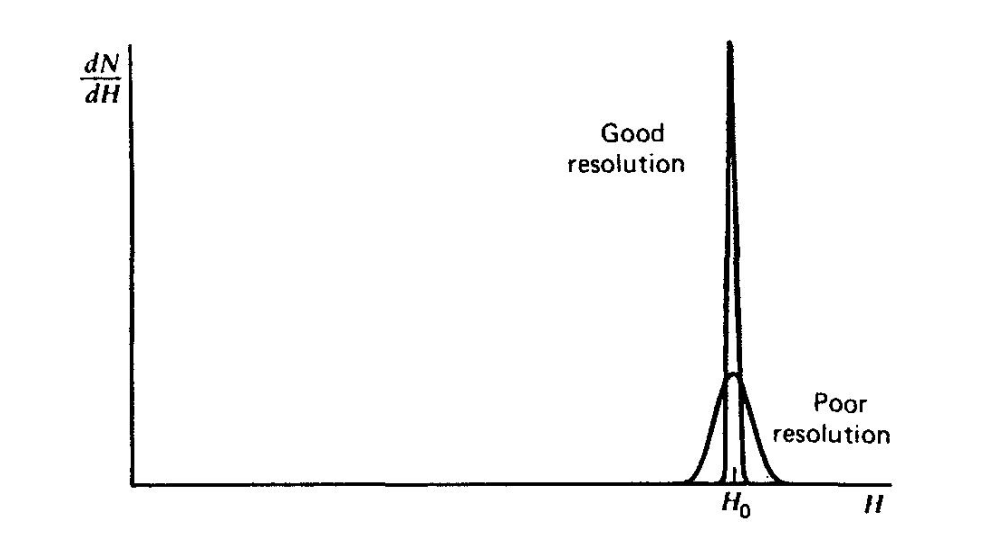
\includegraphics[width=0.6\textwidth]{em4-energetickerozlisenie.png}
\caption{Príklad odozvy pre detektor s dobrým a zlým energetickým rozlíšením.}
\label{em4:img:energetickerozlisenie}
\end{figure}

Dôležité vlastnosti detektorov pri spektroskopickom meraní môžu byť testované zaznamenávaním odozvy na monoenergetický zdroj žiarenia. Rozdelenie diferenciálnych výšok pulzov produkovaných detektorom za týchto podmienok zobrazuje obrázok \ref{em4:img:energetickerozlisenie}. Toto rozdelenie je nazývané \textit{response funkciou} (funkce odezvy) detektoru. V oboch prípadoch bolo detekované rovnaké množstvo pulzov a plochy pod oboma píkmi sú zhodné. Napriek tomu, že sú obe rozdelenia ustrednené na rovnakú priemernú hodnotu $H_0$, šírka rozdelenia detektoru so zlým rozlíšením je o dosť väčšia. To odráža fakt, že od pulzu k pulzu bolo detekované veľké množstvo fluktuácií napriek tomu, že v detektore bola deponovaná tá istá energia pre každý event. Ak sa zmenší množstvo týchto fluktuácií, šírka odpovedajúceho rozdelenia sa tiež zmenší a pík bude viac pripomínať matematickú delta funkciu. Schopnosť pri danom meraní rozlíšiť väčšie detaily rozloženia energie častíc žiarenia sa teda evidentne zlepšuje so zmenšujúcou sa šírkou response funkcie.

\begin{figure}[h]
\centering
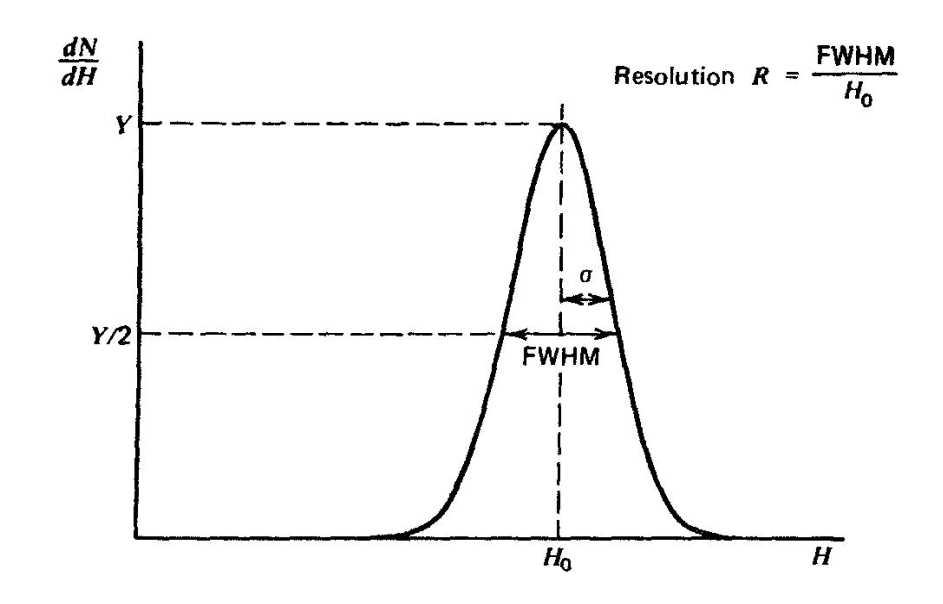
\includegraphics[width=0.6\textwidth]{em4-fwhm.png}
\caption{Pre píky, ktoré majú Gaussovský tvar so štandardnou odchýlkou $\sigma$, je FWHM dané $2,35\sigma$.}
\label{em4:img:fwhm}
\end{figure}

Formálna definícia energetického rozlíšenia detektoru je zobrazená na obr. \ref{em4:img:fwhm}. Plná šírka v polovici výšky (FWHM) je definovaná ako šírka rozdelenia v úrovni, ktorá je polovicou maxima píku. Táto definícia tak úplne zanedbáva vplyv pozadia, na ktoré sa môže pík superponovať. Konvenčne je energetické rozlíšenie bezrozmernou veličinou udávanou v percentách, ktorá sa definuje ako podiel FWHM ku polohe píku $H_0$, Napr. polovodičové detektory používané ku spektroskopii alfa častíc majú energetické rozlíšenie menšie než $1\%$, zatiaľ čo scintilačné detektory používané pre detekciu gama žiarenia majú rozlíšenie $5-10\%$. Je teda jasné, že čím menšie energetické rozlíšenie daný detektor má, tým lepšie bude schopný rozlíšiť dve častice, ktorých energie ležia blízko seba. 

\begin{figure}[h]
\centering
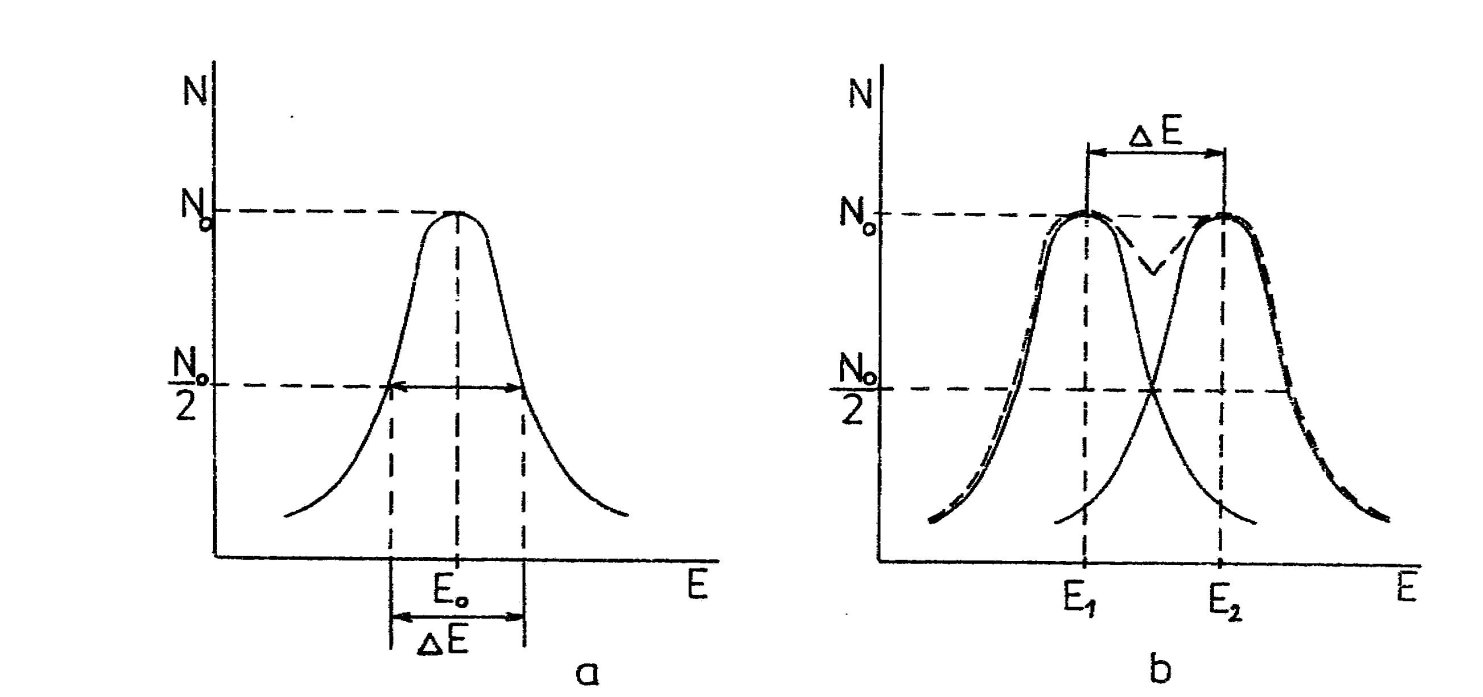
\includegraphics[width=0.8\textwidth]{em4-energetickerozlisenie2.png}
\caption{Rozdelenie kinetickej energie častíc (a) vysielaných monoenergetickým zdrojom s energiou $E_0$. $N$ je početnosť častíc. Rozdelenie dvoch ešte rozlíšiteľných skupín častíc (b) s energiami $E_1$ a $E_2$ a šírkou rozdelení $\Delta E$. Čiarkovaná krivka je súčtová krivka oboch spektrálnych čiar.}
\label{em4:img:energetickerozlisenie2}
\end{figure}

Ak je teda energia častice $E_0$ rozdelená s pološírkou $\Delta E$ (viď obr. \ref{em4:img:energetickerozlisenie2}), je relatívne energetické rozlíšenie $R$ dané vzťahom
\begin{equation}
R=\dfrac{\Delta E}{E_0}.
\end{equation}
Pološírka $\Delta E$ navyše udáva aj možnú polohu ďalšej spektrálnej čiary, ktorú možno zariadením s daným rozlíšením ešte od susednej odlíšiť.

Všeobecne je energetické rozlíšenie funkciou energie deponovanej v detektore, ktorá sa zlepšuje so zvyšujúcou sa energiou. Tento fakt je daný Poissonovým rozdelením ionizácií a excitácií. Stredná energia potrebná k produkcii jedného ión-elektrónového páru je hodnota $w$ závislá iba na materiály. Pre energiu $E$ tak môžeme očakávať $N=\frac{E}{w}$ ionizácií. So zvyšujúcou sa energiou rastie počet ionizačných eventov, čoho výsledkom sú menšie relatívne fluktuácie.

Pre počítanie fluktuácií je treba zvážiť dva prípady. Pre detektor, kde žiarenie nie je celkom pohltené, je počet ionizačných interakcií daný Poissonovským rozdelením. Odchýlka tohto rozdelenia je daná
\begin{equation}
\sigma = \sqrt{N},
\end{equation}
kde $N$ je stredný počet párov produkovaných ionizáciou. Relatívne energetické rozlíšenie je tak dané
\begin{equation}
R=2,35\dfrac{\sqrt{J}}{J}=2,35\sqrt{\dfrac{w}{E}},
\end{equation}
kde faktor $2,35$ vzťahuje štandardnú odchýlku Gaussiánu k jeho FWHM. 

Ak je absorbovaná celá energia žiarenia, ako v detektoroch používaných ku spektroskopickým meraniam, predpoklad Poissonovského rozdelenia nie je správny. V mnohých detektoroch je energetické rozlíšenie pozorované menšie než to určené z Poissonovho rozdelenia. Rozdiel je v tom, že celková deponovaná energia je fixná, zatiaľ čo v predchádzajúcom prípade mohla deponovaná energia fluktuovať. Celkový počet ionizácií a energia ionizujúcej častice stratená v každej interakciu sú zviazané touto hodnotou. Štatisticky to znamená, že ionizačné eventy nie sú všetky nezávislé, a preto Poissonovo rozdelenie nemožno aplikovať. Prvým, kto spočítal odchýlku za týchto podmienok, bol Ugo Fano a odvodil
\begin{equation}
\sigma = \sqrt{FN}
\end{equation}
kde $N$ je stredný počet produkovaných ionizačnách párov a $F$ je \textbf{Fano faktor.}

Fano faktor je funkcia všetkých fundamentálnych procesov, ktoré môže viesť k prenosu energie v detektore, zahrňujúce všetky reakcie, ktoré nemusia viesť k ionizácií (napr. fotónové excitácie). Je to teda konštanta charakterizujúca detekujúce médium. Teoreticky je veľmi obtiažne Fano faktor určiť, pretože to vyžaduje podrobnú znalosť všetkých reakcií, ktoré môžu nastať v detektore.

S použitím Fano faktoru je relatívne energetické rozlíšenie dané
\begin{equation}
R=2,35\sqrt{\dfrac{Fw}{E}}
\end{equation}
Pre $F=1$ je rozptyl rovnaký, ako pre Poissonove rozdelenie. To je prípad scintilačných detektorov. Pre množstvo detektorov, polovodičových či plynových, je $F<1$, čo veľmi zvyšuje energetické rozlíšenie týchto typov detektorov. Hodnoty pre niekoľko materiálov sú uvedené v tabuľke \ref{em4:tab:fano}.

\begin{table}[h]
\centering
\begin{tabular}{l|c}
Materiál & Fano faktor \\ \hline
Kremík & 0,09 \\
Germánium & 0,06 \\
Argón & 0,20 \\
Xenón & 0,13 
\end{tabular}
\caption{Hodnoty Fano faktoru pre niekoľko materiálov.}
\label{em4:tab:fano}
\end{table}

Fano faktor odráža mieru, ktorou sa energia interagujúcej častice premieňa na nosiče informácie v detektore. Ak bude energia vstupujúceho žiarenia vždy premenená na iónové páry, potom ich počet bude vždy presne rovnaký bez akýchkoľvek štatistických fluktuácií - v takom prípade bude $F=0$. Naopak ak sa len malá časť energie žiarenia bude podieľať na tvorbe páru, ktoré teda vznikajú len s malou pravdepodobnosťou, budú dobre splnené podmienky pre Poissonovo rozdelenie, potom $\sigma=\sqrt{N}$ a $F=1$.

\subsection{Detekčná účinnosť}

Predstavme si opäť náš hypotetický detektor. V princípe pre každú časticu, ktorá interaguje v priestore detektoru, dá tento detektor odozvu. Primárne častice (ako napr. alfa či beta častice) spôsobujú excitáciu alebo ionizáciu ihneď po vstupe do aktívneho objemu detektoru a po tom, čo prejdú časťou dráhy svojho dosahu, vytvoria dostatok iónových párov pozdĺž svojej dráhy, aby výsledný pulz bol dostatočne veľký k zaznamenaniu. Preto si možno jednoducho predstaviť situáciu, kedy je detektor schopný zaznamenať každú nabitú častice, ktorá vstúpi do jeho objemu. Pri týchto podmienkach je detekčná účinnosť $100\%$.

Na druhej strane ale pre častice bez náboja (ako napr. gama žiarenie alebo neutróny) je situácia zložitejšia, nakoľko tieto častice musia najskôr zinteragovať v objeme detektoru a vytvoriť sekundárnu nabitú časticu. Detektory neutrálnych častíc tak často mávajú účinnosť nižšiu než $100\%$. Potom je treba mať presný údaj o efektivite detektoru , aby bolo možné vztiahnuť počet zaznamenaných pulzov k počtu neutrónov či fotónov gama žiarenia, ktoré vnikli do detektoru.

Detekčnú účinnosť môžeme rozdeliť na dva druhy: totálnu a vnútornú. Totálna detekčná účinnosť $\eta_{tot}$ je podiel počtu zaznamenaných pulzov k počtu častíc emitovaných zdrojom a berie tak do úvahy nielen vlastnosti detektoru, ale aj geometriu. Vnútorná účinnosť $\eta_{in}$ dáva do podielu počet zaznamenaných pulzov k počtu častíc prichádzajúcich do detektoru. Táto účinnosť nezávisí na geometrii, ale na materiály, energii žiarenia a hrúbke detektoru v smere, v ktorom žiarenie prichádza. Obe účinnosti sú jednoducho previazané vzťahom
\begin{equation}
\eta_{tot}=\eta_{in}\dfrac{S}{4\pi d}
\end{equation}
kde $S$ je plocha detektoru a $d$ je vzdialenosť zdroja a detektoru. Pomer $\frac{S}{4\pi d}$ označujeme za geometrickú účinnosť $\eta_{geom}$ (podíl počtu částic dopadlých na detektor a počtu částic vyzářených zdrojem).

Príčiny toho, že niektoré častice nie sú registrované a účinnosť je menšia než očakávaných $100\%$, môžu byť:
\begin{itemize}
\item častica pri svojom prechode citlivým objemom nevytvorí ani jeden ión-elektrónový pár
\item častica vytvorí iba malý počet ión-elektrónových párov, ktorých signál neprekročí nastavenú hodnotu diskriminačnej hladiny
\item časový interval, v ktorom došlo k interakcii dvoch či viacerých po sebe interagujúcich častíc, bol kratší, než rozlišovacia doba detektoru a/alebo elektroniky zaisťujúcej registráciu. V takom prípade účinnosť detekcie klesá s rastúcou početnosťou.
\end{itemize}

\subsection{Mŕtva doba}

Prakticky vo všetkých detektoroch je pre detekciu dvoch po sebe idúcich eventov ako dvoch odlišných pulzov nutné, aby tieto eventy od seba boli oddelené istým časom. V niektorých prípadoch je tento limitujúci čas daný detektorom ako takým, inokedy napr. elektronikou. Minimálne časové odlíšenie je nazývané \textbf{mŕtva doba} systému. Straty kvôli mŕtvej dobe sú vážne najmä pri vysokých početnostiach častíc žiarenia.

Mŕtva doba je doba potrebná pre vytvorenie a spracovanie signálu v detektore. Existujú dve možnosti, ako sa môže detektor behom mŕtvej doby chovať: buď sa stane necitlivým k ďalším prichádzajúcim časticiam, alebo zostáva citlivý a vzniká tzv. \textbf{pile-up} efekt, t.j. skladanie amplitúd prichádzajúcich častíc.

V prípade, že sa mŕtva doba nepredĺži, platí pre skutočný počet častíc vzťah
\begin{equation}
N_s=nT=mT+nmT\tau,
\end{equation}
kde $n$ je skutočná početnosť, $T$ je doba merania, $m$ je početnosť zaznamenaných prípadov, a $\tau$ je mŕtva doba. Skutočný počet tak môžeme jednoducho vyjadriť ako
\begin{equation}
N_s=\dfrac{mT}{1-m\tau}.
\end{equation}

V prípade modelu, kedy sa mŕtva doba predlžuje a vznika pile-up efekt môžeme nameranú početnosť vyjadriť ako
\begin{equation}
m=ne^{-n\tau}.
\end{equation}

Pre oba modely platí, že pre nízke početnosti ($n\ll 1/\tau$) sa nameraná početnosť dá aproximovať do rovnakého tvaru:
\begin{equation}
m=\dfrac{n}{1+n\tau}\approx n(1-n\tau) \approx	ne^{-n\tau}.
\end{equation}

Mŕtva doba je teda čas, ktorý musí prejsť medzi registráciou jednej častice a schopnosťou reagovať na ďalšiu časticu. Mŕtva doba, počas ktorej nie sú detekované žiadne častice, je nasledovaný fázou, počas ktorej sú častice opäť detekované, avšak detektor nemusí odpovedať na častice s plnou citlivosťou. Po určitom čase, nazývanom doba zotavenia (\textit{recovery time}), detektor dokáže opäť vytvárať signál s normálnou amplitúdou (viď obr. \ref{em4:img:mrtvadoba}).

\begin{figure}[h]
\centering
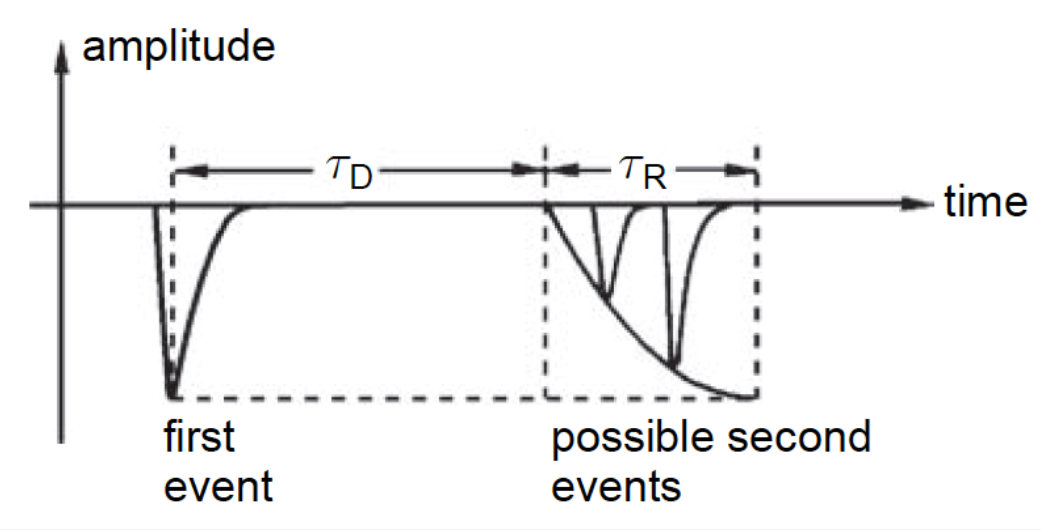
\includegraphics[width=0.7\textwidth]{em4-mrtvadoba.png}
\caption{Ukážka mŕtvej doby a doby zotavenia v Geiger-Mullerovom počítači.}
\label{em4:img:mrtvadoba}
\end{figure}

\section{Plynové detektory}

Za štandardných laboratórnych podmienok sa plyny chovajú ako veľmi dobré až vynikajúce izolanty. Pôsobením priamo ionizujúceho žiarenia sa niektoré atómy alebo molekuly, pôvodne neutrálne, premieňajú ionizáciou na kladne nabité ióny a elektróny. Pri interakcii nepriamo ionizujúceho žiarenia túto ionizáciu spôsobujú sekundárne nabité častice. Dôsledkom toho vodivosť plynu narastá. Detektory využívajúce tohto javu sa označujú ako plynové detektory. Patria k nim nasledujúce:
\begin{itemize}
\item ionizačné komory
\item proporcionálne komory
\item Geige-M\"{u}llerove detektory
\item koronové detektory
\end{itemize}
Tieto detektory sa od seba vzájomne líšia predovšetkým veľkosťou a rozložením intenzity elektrického poľa (určeným geometriou detektoru a napájacím napätím podľa vzťahu $E=\frac{U}{d}$) a druhom a tlakom pracovného plynu.

Plynovou náplňou komory môže byť v princípe aj obyčajný vzduch, lepšie vlastnosti však vykazujú špeciálne plynové náplne tvorené inertnými chemicky stabilnými plynmi, ktorých molekuly nepodliehajú pri prechode elektrického prúdu chemickým premenám. Najčastejšie sa používa argón, kryptón a xenón.

\begin{figure}[h]
\centering
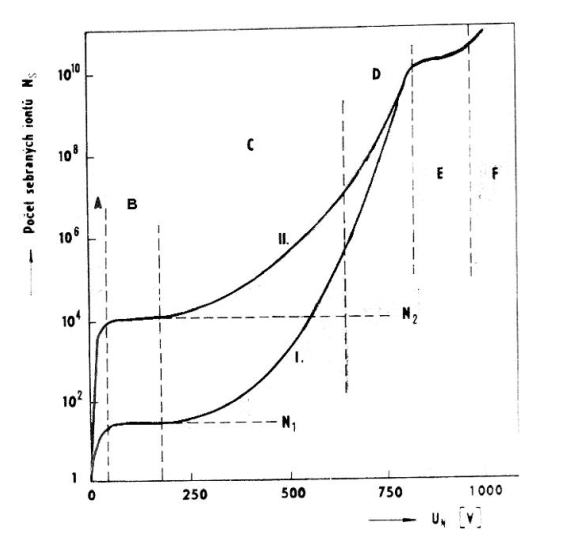
\includegraphics[width=0.7\textwidth]{em4-plynovedetektory.png}
\caption{Závislosť počtu zozbieraných iónov na napätí detektoru.}
\label{em4:img:plynovedetektory}
\end{figure}

Všeobecný priebeh charakteristiky plynového detektoru je na obr. \ref{em4:img:plynovedetektory} a zobrazuje počet iónov $N_s$ zozbieraných na elektródach počítača v závislosti na pripojenom napätí a teda intenzite elektrického poľa. Krivka I odpovedá častici, ktorá vnútri pracovného objemu detektoru vytvorí $N_1$ iónových párov, krivka II potom iné častice, ktoré vytvoria $N_2>N_1$ iónových párov. Je zrejmé, že táto druhá častica zanechala v detektore vyššiu energiu.

V oblasti A v dôsledku nedostatočnej intenzity elektrického poľa nie sú od seba produkty ionizácie dostatočne rýchlo oddelené a dochádza k ich rekombinácii. Celkový zozbieraný náboj je preto menší, než odpovedá ionizáciou vytvorenému náboju, túto oblasť nazývame \textit{rekombinačnou oblasťou}. S rastúcou intenzitou elektrického poľa rastie aj driftová rýchlosť vytvorených nosičov náboja, pohybujúcich sa k príslušným elektródam a pravdepodobnosť rekombinácie klesá natoľko, že sa od istej hodnoty napätia na detektore už prakticky neuplatňuje. Počet zozbieraných nosičov náboja $N_s$ sa rovná počtu nosičov vytvorených ionizáciou. Oblasť označená B sa nazýva \textit{oblasť nasýtenia}. Zatiaľ čo oblasť A nie je prakticky používaná, oblasť B je typickým pracovným režimom ionizačných komôr.

Pri ďalšom zvyšovaní napätia na detektore je počet zozbieraných nosičov náboja $N_s$ väčší než odpovedá $N_1$ či $N_2$, pričom konštanta úmernosti $M$ je iba funkciou napätia na detektore a označuje sa ako plynové zosilnenie (platí $N_s=MN_{1/2}$). Táto oblasť, kde plynové zosilnenie $M$ nezávisí na veľkostiach $N_1$ či $N_2$, sa nazýva \textit{oblasť proporcionality} a je typickým režimom proporcionálnych detektorov.

Pri ďalšom zvyšovaní napätia sa plynové zosilnenie $M$ stáva funkciou nielen napätia, ale aj $N_1$ a $N_2$ - túto oblasť (D) nazývame \textit{oblasť obmedzenej proporcionality} a nie je bežné používaným režimom plynových detektorov.

S ďalším zvyšovaním napätia na detektore obe krivky splývajú v jedinú ďalej rastúcu krivku. Oblasť označená E a charakterizovaná nezávislosťou odozvy na veľkosti pôvodne vytvorených ionizácií a iba veľmi pozvoľnou závislosťou na ďalšom zvyšovaní napätia sa nazýva \textit{Geiger-M\"{u}llerova oblasť} a pracujú v nej Geiger-M"ullerove detektory. Pri ďalšom zvyšovaní napätia dochádza k zapáleniu samovoľného koronového výboja (oblasť F).

Ako ionizačná komora, tak aj proporcionálny detektor umožňuje meranie energie častíc a hovoríme, že majú spektrometrické vlastnosti. Oproti tomu napr. Geiger-M"ullerov počítač udáva iba informáciu o detekcii častice, z jeho odozvy nemožno určiť energiu častíc.

Dôležité je tiež zdôrazniť, že k dosiahnutiu oblasti proporcionality a ďalších oblastí ležiacich na obr. \ref{em4:img:plynovedetektory} vpravo od nej je nutné použiť geometrického usporiadania detektoru, ktoré zaistí veľmi nehomogénne elektrické pole (najčastejšie sa používa koaxiálna geometria, niekedy tiež sférická).

\subsection{Ionizačné komory}

Hlavné využitie nachádzajú ionizačné komory v dozimetrii pri stanovení veličín expozícia, kerma a dávka. Komora je naplnená vzduchom, najčastejšie geometrickým tvarom je dosková či valcová, zriedka sférická. Schopnosť práce ionizačných komôr za vysokých teplôt je bezkonkurenčná, žiadny z ostatných známych detektorov túto vlastnosť nemá.

Vyhodnotenie odozvy ionizačnej komory možno spraviť buď v prúdovom alebo v impulznom režime. Straty pri detekcii častíc v ionizačnej komore sú najmä vplyvom rekombinácie (či už elektrón-iónovej, alebo rekombinácie medzi záporným a kladným iónom - v oboch prípadoch je náboj reprezentujúci pôvodne vytvorený pár stratený a nemôže prispieť ku vzniku signálu v detektore) a difúzia (tá sa deje v smere klesajúceho gradientu a spôsobuje pohyb nábojov proti smeru, ktorým sa pohybuje vplyvom elektrického poľa). Najjednoduchšou cestou ku zníženiu týchto strát je použite vysokých hodnôt napájacieho napätia komory.

Elektrický prúd pretekajúci ionizačnou komorou je všeobecne veľmi slabý (cca $10^{-16}$ až $10^{-9}$~A) - ionizačná komora má nízku citlivosť, takže sa nehodí na detekciu slabého toku žiarenia. Jej výhodou je však lineárna závislosť prúdu aj v oblasti vysokých intenzít ionizujúceho žiarenia. Ionizačné komory preto majú veľmi dobrú linearitu odozvy na intenzitu detekovaného ionizujúceho žiarenia vo veľmi širokom rozsahu. Využíva sa preto napr. na meranie rozloženia intenzity vo zväzkoch žiarenia v rádioterapii. Najčastejšie použitie ionizačnej komory je v dozimetrii na meranie dávky ionizujúceho žiarenia.

\subsection{Proporcionálne komory}

Tento typ plynových detektorov využíva jav nazývaný \textbf{plynové zosilnenie} ku znásobeniu počtu nosičov náboja vytvorených ionizáciou v plyne. Pracuje takmer vždy v impulznom režime (výstupné impulzy majú vďaka plynovému zosilneniu podstatne väčšie amplitúdy než u impulzne pracujúcich ionizačných komôr).

Plynové zosilnenie, ktoré sa odohráva vo veľmi blízkom okolí anódy, je závislé na intenzite elektrického poľa a začína sa za normálneho atmosférického tlaku uplatňovať v plynoch nevytvárajúcich záporné ióny od hodnôt intenzity elektrického poľa $10^6\:\unit{V/m}$. Elektróny vytvorené primárnou ionizáciou sú elektrickým poľom urýchlené natoľko, že spôsobujú na svojej dráhe ionizáciou neutrálnych atómov či molekúl plniaceho plynu. Týmto vznikajú ďalšie elektróny, ktoré sú poľom taktiež urýchľované a ak dosiahnu vyššie energie, než je ionizačná energia neutrálnej molekuly, môžu plynovú náplň sami ionizovať. V dôsledku toho počet ión-elektrónových párov rastie a vznika tzv. \textbf{Townsendova lavína}.

Rozloženie elektrického poľa obzvlášť v okolí anódy môže podstatne ovplyvniť priestorový náboj kladných iónov, ktoré sa pohybujú ku katóde rýchlosťou podstatne menšou, než elektródy k anóde. Dôsledkom je zníženie amplitúdy signálu a negatívny vplyv na energetickú rozlišovaciu schopnosť detektoru.

Proporcionálne detektory sa odporúčajú prevádzkovať pri najnižšom možnom napätí, za ktorého dochádza k plynovému zosilneniu. Je to kvôli ohľadu na potlačenie vplyvu priestorového náboja a šumu detektora.

\subsection{Geiger-M"ullerove detektory}

Ak ďalej zvyšujeme napájacie napätie, od istej hladiny budú v dôsledku veľkej intenzity elektrického poľa v oblasti anódy elektrónové lavíny natoľko urýchlené, že okrem nárazovej ionizácie môžu tiež excitovať atómy alebo molekuly plynovej náplne. Deexcitáciu sprevádza emisia fotónového žiarenia. Tieto fotóny sa z miesta svojho vzniku šíria všetkými smermi, môžu teda dopadnúť na ktorékoľvek miesto katódy. Ak je ich energia väčšia ako výstupná práca elektrónu z kovového povrchu, na ktorý dopadnú, dôjde k emisii fotoelektrónu. Tie sa účinkom poľa pohybujú k anóde, v ktorého okolí spôsobia vznik ďalších lavín a celý proces sa opakuje. Zásluhou fotoelektrónov sa tento Geiger-M"ullerov výboj z miesta primárnej ionizácie rozšíri pozdĺž celého počítača.

Nasleduje však zníženie intenzity elektrického poľa vďaka pôsobenie priestorového náboja kladných iónov, ktoré vo forme trubice obalia anódu po celej jej dĺžke. V dôsledku tohto zníženia intenzity elektrického poľa elektróny prestanú excitovať plynovú náplň, ustane tvorba deexcitačných fotónov, na katóde prestanú vznikať fotoelektróny a výboj v počítači ustáva. 

Následne ale v detektore vzniká sekundárna lavína. Deje sa tak vďaka tomu, že vrstva kladných iónov, ktoré pôvodne obaľovali anódu, sa pohybuje ku katóde počítača, na ktorého povrchu sa ióny neutralizujú záchytom elektrónov. Pritom je energeticky možná emisia voľného elektrónu z katódy, ktorý za dobu niekoľko mikrosekúnd dosiahne anódy a spustí sekundárnu lavínu. Výsledkom prvotnej ionizácie jedinou časticou tak nie je jeden impulz, ale nepretržitá séria impulzov. Aby mohol počítač registrovať jednotlivé nabité častice prechádzajúce jeho objemom ako jednotlivé impulzy, je treba predísť vzniku sekundárnych lavín. Tento proces sa nazýva zhášanie a podla neho sa Geiger-M"ullerove počítače delia na
\begin{itemize}
\item \textbf{nesamozhášacie} - jedinou možnosťou zhášania u nich je zmenšenie intenzity elektrického poľa znížením napájacieho napätia pod hodnotu prahového napätia
\item \textbf{samozhášacie} - bolo zistené, že samovoľné zhášanie výboja spôsobuje prímes alkoholových pár v inak bežne používaných vzácnych plynoch. Pri neutralizácií kladných iónov zhášacej prímesy na katóde sa uvoľnená energia využije oveľa pravdepodobnejšie k disociácii ich zložitých molekúl než k uvoľneniu elektrónu z povrchu katódy, a preto nedochádza ku spusteniu sekundárnych lavín. Fotoelektróny sú naviac produkované v atómoch zhášajúcej prímesy, čím sa predíde rozšíreniu výboja pozdĺž celého počítaču. Nevýhodou organických zhášacích prímesí je obmedzenie životnosti počítača spôsobené postupným znižovaním počtu neutrálnych molekúl zhášacieho plynu behom doby jeho používania, nakoľko jeho už disociované molekuly nie sú schopné regenerácie na pôvodnú molekulu. Oproti tomu molekuly halogénov pri zhášaní počítača majú schopnosť opäť rekombinovať na neutrálnu molekulu.
\end{itemize}

Ako je vidieť na obr. \ref{em4:img:plynovedetektory}, Geiger-M"ullerove počítače pracujú v oblasti, kde nárast napätia je nasledovaný len malým stúpaním nameranej početnosti. Táto oblasť sa nazýva \textit{pracovnou plošinou} počítača. Jej dĺžka a sklon sú meradlami kvality počítača a závisí na jeho type, predchádzajúcej histórii a teplote. Počiatočné napätie odpovedá takej intenzite elektrického poľa, pri ktorej deexcitačné fotóny zaistia pokračovanie výboja generáciou dostatočného počtu fotoelektrónov.

Priestorový náboj kladných iónov, obalujúci ako trubice anódu počítača po celej jej dĺžke, znižuje intenzitu elektrického poľa v jej okolí natoľko, že elektróny pochádzajúce z ďalšej interakcie registrovaného žiarenia nevytvoria lavíny. Tento stav trvá tak dlho, pokiaľ sa driftujúce kladné ióny nedostanú do takej vzdialenosti od anódy, aby pole v jej okolí dosiahlo kritickej intenzity potrebnej pre tvorbu lavín. Tento časový interval sa nazýva mŕtva doba. Čas medzi koncom mŕtvej doby a okamžikom zberu kladných iónov je doba zotavenia.

Detekčná účinnosť GM detektorov všeobecne závisí na stenách detekčnej trubice a na jej plynovej náplni. Diametrálne sa líši pre žiarenie tvorené nabitými časticami a pre fotónové žiarenie. Pre ťažšie nabité častice (napr. $\alpha$) a pre elektróny je detekčná účinnosť blízka $100\%$ za predpokladu, že sa dostanú do plynovej náplne, t.j. do citlivého objemu detektoru. Aby tam prenikli, musí byť vstupné okienko z čo najtenšieho ľahkého materiálu\footnote{hovorí sa o \quotedblbase bezokienkových\textquotedblright ~detektoroch}. Pre fotónové žiarenie je detekčná účinnosť vlastnej plynovej náplne veľmi nízka, vzhľadom k jeho malej absorpcii v plyne. Naprostá väčšina $\gamma$ fotónov prejde citlivým objemom plynu bez interakcie. Fotóny s vyššou energiou môžu byť detektorom s plynovou náplňou detekované prakticky iba vtedy, keď budú interagovať s materiálom steny detekčnej trubice.

GM detektory zohrali významnú úlohu v rozvoji jadrovej a radiačnej fyziky - bol to prvý typ detektorov, ktorý dokázal registrovať jednotlivé kvantá ionizujúceho žiarenia a nielen iba intenzitu či tok žiarenia ako je to pri obyčajných ionizačných komorách. Aj v súčasnej dobe sú GM detektory používané pre svoju jednoduchosť, avšak väčšinou iba na menej náročné merania. Napr. v radiačnej ochrane sú to merače kontaminácie, hlásiče radiácie, monitorovacie systémy a pod. Pre presnejšie a náročnejšie merania boli vytlačené predovšetkým scintilačnými a polovodičovými detektormi, ktoré sú síce mnohonásobne drahšie, avšak majú po všetkých stránkach podstatne lepšie parametre.


\section{Scintilačné detektory}

Scintilačné detektory prevádzajú absorbovanú energiu ionizujúceho žiarenia na energiu fotónov s frekvenciou v oblasti viditeľného alebo ultrafialového svetla. Historicky ide o najstarší spôsob detekcie jednotlivých ťažkých nabitých častíc, kedy záblesky tienidla pokrytého vrstvou ZnS boli počítané pomocou jednoduchého mikroskopu okom pozorovateľa. Toto zariadenie sa nazývalo spintariskop a kládlo na zrak pozorovateľa značné nároky. V roku 1909 uskutočnili Geiger a Marsden pomocou spintariskopu experiment zaoberajúci sa rozptylom $\alpha$ častíc na tenkej fólii, ktorý viedol k Rutherfordovmu objavu jadra (1911). V tejto súvislosti sa hovorí, že Marsden, ktorý scintilácie počítal (a boli ich státisíce), mal Geigerom prísne zakázané pozerať sa von oknom a tráviť čas vonku v dobe ostrého slnečného svetla, aby sa nezhoršili jeho schopnosti \quotedblbase ľudského scintilačného počítača\textquotedblright .

Je udivujúce, že navzdory subjektivite tejto detekčnej metódy stanovil Regener nielen počet $\alpha$ častíc emitovaných jedným gramom Ra a Po, ale tiež zo známeho toku častíc nabíjajúcich kondenzátor, po zmeraní celkového náboja, určil náboj $\alpha$ častice s chybou menšou než $0,375\%$ jeho súčasnej tabuľkovej hodnoty.

Už v roku 1941 sa pokúsil Krebs využiť fotocitlivého Geiger-M\"ullerovho detektoru ako náhrady ľudského zraku pri počítaní scintilácií ZnS tienidla. Napriek tomu, že sa o to isté pokúšalo viacero autorov, výsledky neboli dobré. Nevýhod takto aplikovaného GM detektoru bolo mnoho. Medzi hlavné patrila nevýhodne položená oblasť maxima spektrálnej citlivosti (cca 260 nm), schopnosť detekcie no nie spektrometrie, neschopnosť rozlíšenia druhu častice podľa odozvy a napokon veľká mŕtva doba rádu $10^{-4}$ s.

Prvý prakticky využiteľný scintilačný detektor vznikol (1944) v Los Alamos National Laboratory (USA), kedy Curran a Baker použili na detekciu svetelných zábleskov ZnS fotonásobiče firmy RCA typu 1P 21, vyvinutého pre fotometrické účely vo filmovom priemysle.

K prevratu, ktorý znamenal návrat scintilačného detekčného  princípu do experimentálnych laboratórií došlo po roku 1947, kedy boli v rýchlom slede objavené scintilačné vlastnosti organických\footnote{antracén - 1947, Kallmann} aj anorganických\footnote{NaI(Tl) - 1948, Hofstadter} látok. Tieto objavy stimulovali výrobcov k vývoju vhodnejších fotonásobičov. Rýchly vývoj nových scintilátorov bol v podstate ukončený objavmi plastikových a kvapalných scintilátorov v roku 1950. Až koncom šesťdesiatych rokov bol uvedený a ďalej vyvíjaný nový scintilátor BGO s vysokým protónovým číslom $Z=83$. NaI(Tl) však zostal dodnes najpoužívanejším scintilačným detektorom fotónového žiarenia s najlepšou energetickou rozlišovacou schopnosťou.

Scintilačné detektory patria medzi najpoužívanejšie detektory ionizujúceho žiarenia. Ich výhoda spočíva okrem dobrých spektrometrických vlastností tiež v tom, že detekčné médium, scintilátor, môže mať značné rozmery a takmer ľubovoľný tvar. Pritom hmotnosť scintilačných látok je dostatočne veľká, takže možno dosiahnuť pomerne veľkú detekčnú účinnosť, najmä pre gama žiarenie. Scintilačný detektor tiež dáva výstupný signál, ktorého ďalšie spracovanie obvykle nevyžaduje použitie veľmi citlivých zosilňovačov. Vzhľadom k rýchlej odozve sa scintilačné detektory uplatňujú tam, kde je rozhodujúcim činiteľom spracovanie veľkých početností alebo kde potrebujeme získať informácie o časových vzťahoch emisie častíc.

Základné usporiadanie scintilačného detekčného systému je znázornené na obr. \ref{em4:img:schemascint}. Vlastné čidlo detektoru predstavuje scintilátor, v ktorom dopadajúce žiarenie spôsobuje ionizáciu a excitáciu jeho atómov a molekúl. Ich návrat do základného stavu je doprevádzaný emisiou svetelného žiarenia. Aby sa mohli svetelné fotóny maximálne využiť, obklopuje sa scintilátor \textit{reflektorom}. Zozbierané fotóny po prechode optickým kontaktom pôsobia na fotokatódu fotonásobiča. Fotóny po dopade na fotokatódu uvoľňujú fotoelektróny, ktoré sa po fokusácií a urýchlení elektrickým poľom dostávajú na prvú dynódu. Povrch dynód je pokrytý materiálom s veľkým súčiniteľom sekundárnej emisie. Vplyvom toho sa počet elektrónov opúšťajúcich každú nasledujúcu dynódu neustále zväčšuje. Výsledkom tohoto násobiaceho procesu je, že každý fotoelektrón vyvolá celkom $s$ elektrónov, ktoré sú potom zozbierané na anóde fotonásobiča. Zosílenie fotonásobiča býva v rozsahu $10^5$ až $10^9$.

\begin{figure}[h]
\centering
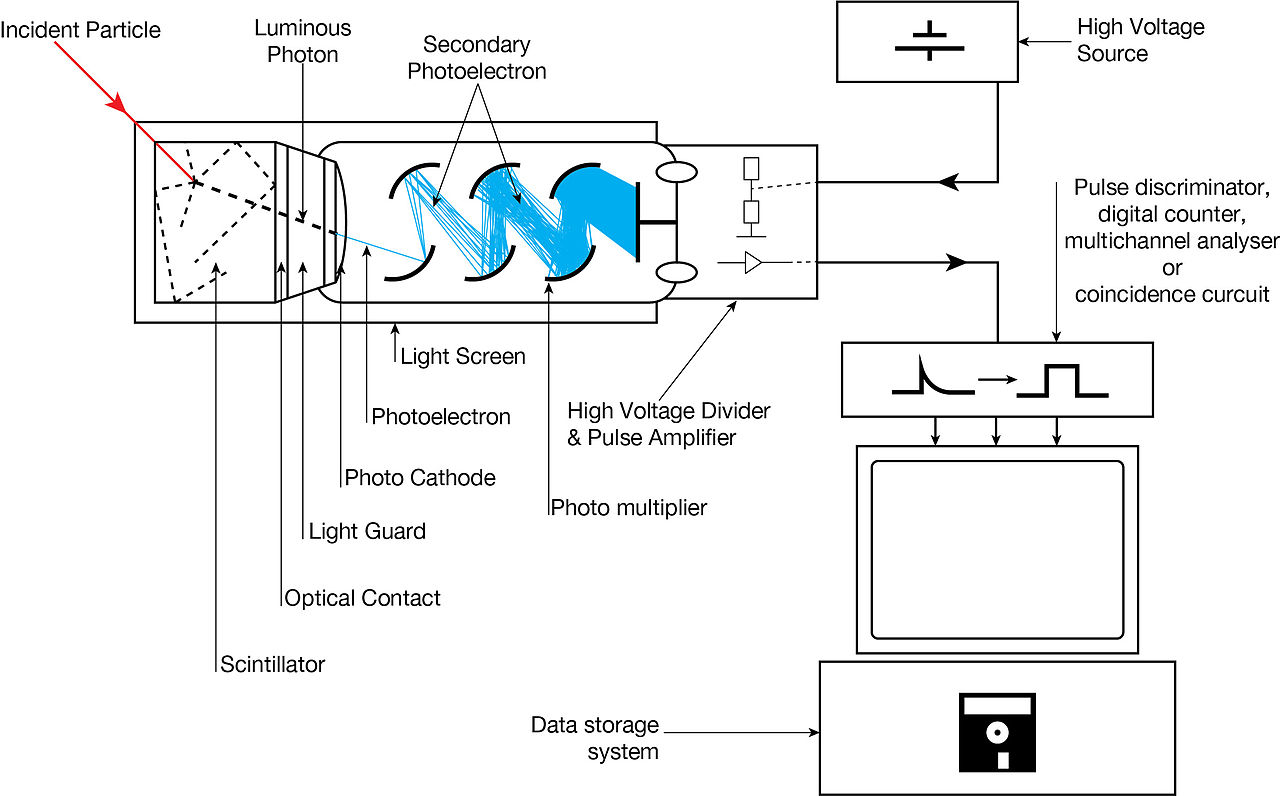
\includegraphics[width=0.7\textwidth]{js1-scint.jpg}
\caption{Schéma scintilačného detektoru.}
\label{em4:img:schemascint}
\end{figure}

Od vhodných scintilačných materiálov požadujeme nasledujúce vlastnosti: vysoká efektivita premeny kinetickej energie nabitých častíc na scintilačné fotóny, dobrá linearita konverzie - svetelný výťažok by mal byť priamo úmerný uloženej energii pre široké spektrum energií, priehľadnosť pre svoje emisné vlnové dĺžky, emisné spektrum zhodné so spektrálnou citlivosťou fotonásobiča, krátka rozpadová konštanta, dobré optické vlastnosti, dobrá opracovateľnosť, index lomu by mal byť blízky indexu lomu skla ($\sim 1,5$).

\subsection{Organické scintilátory}


Energia ionizujúceho žiarenia v akomkoľvek scintilátore sa prejavuje emisiou fotónov prislúchajúcich do ultrafialovej až viditeľnej časti spektra, ktorá sa označuje ako luminescencia. Tá je v organických scintilátoroch vlastnosťou molekulárnej štruktúry aromatických molekúl a súvisí s energetickými stavmi $\pi$ elektrónov sprostredkujúcich medziatómové väzby v organických molekulách. Pretože tento spôsob väzby nie je závislý na skupenstve, pozorujeme luminescenciu v plynných, kvapalných aj tuhých aromatických látkach.

Celková energia vyžiarených luminescenčných fotónov je prirodzene vždy nižšia, než energia absorbovaná scintilátorom. Ich pomer sa nazýva \textbf{konverzná účinnosť} scintilátoru.

Absorbovaná energia žiarenia sa spotrebuje hlavne na ionizáciu a excitáciu elektrónov materiálu scintilátoru, efekt luminescencie je spojený iba s deexcitáciou $\pi$-elektrónov. Ionizácia iných, než $\pi$-elektrónov vedie k dočasnému alebo aj k trvalému poškodeniu molekúl scintilátoru.

\begin{figure}[h]
\centering
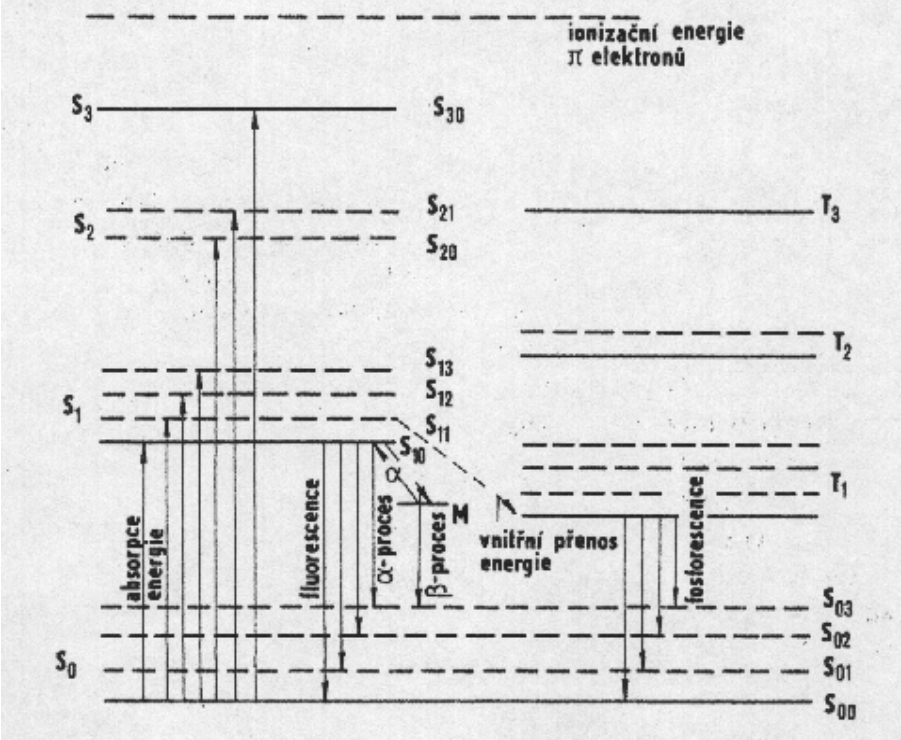
\includegraphics[width=0.7\textwidth]{em4-orgscint.png}
\caption{Schéma energetických stavov $\pi$-elektrónov a názvy luminescencie jednotlivých deexcitačných stavov.}
\label{em4:img:orgscint}
\end{figure}

Ak je $\pi$-elektrón excitovaný priamo alebo prostredníctvom iného elektrónu, prechádza zo základného stavu $S_{0j}$ do excitovaného stavu $S_{ij}$ závislého na veľkosti dodanej energie. Index $i$ označuje excitované singletové stavy, indexom $j$ sú rozlíšené vedľajšie vibračné hladiny $i$-teho singletového stavu. Podobne je to aj pre tripletové stavy $T_{ij}$, ktorých energia je vždy nižšia než energia rovnako indexovaného singletového stavu. Singletový stav odpovedá energetickým hladinám, v ktorých je súčet spinov elektrónov molekuly rovný nule. Tripletový stav má celkový spin $1$. 

Deexcitácia $\pi$-elektrónov môže prebehnúť podľa výberových pravidiel z vyšších excitovaných stavov buď priamo do základného stavu, alebo kaskádovo cez nižšie excitované stavy až do základného stavu. Experimentálne bolo dokázané, že k luminescencii môže dôjsť iba pri prechode zo stavu $S_{10}$ do $S_{0j}$, pričom tento prechod je s istou pravdepodobnosťou nežiarivý. Znamená to, že pri každom prechode medzi oboma zmienenými energetickými stavmi nemusí byť nezbytne vyžiarený fotón. Deexcitačná energia sa v takom prípade mení na teplo, rovnako ako pri všetkých ostatných možných deexcitáciach, ktoré prebehnú inými spôsobmi, než $S_{10}\rightarrow S_{0j}$. O týchto prechodoch potom hovoríme ako o nežiarivých. Prechod $T_{10}\rightarrow S_{0j}$ je spinovo zakázaný, doba života tripletových stavov je preto omnoho väčšia než singletových stavov. Dôsledkom deexcitácií tripletových stavov je veľmi dlhá doba vysvietenia, ktorá je u scintilačného detektoru nežiadúca.

Scintilačné detektory obyčajne nie sú vhodné na detekciu ťažkých iónov. Naopak, detekčná účinnosť elektrónov je v podstate stopercentná. Avšak kvôli tomu, že elektróny sa môžu v látke rozptýliť o veľké uhly, môžu opustiť detektor bez toho, aby zanechali celú svoju energiu. Pri beta žiaričoch sa často používa metóda tzv. vnútorného počítania, vyznačujúca sa veľmi veľkou detekčnou účinnosťou. Metóda spočíva v tom, že rádioaktívna vzorka je rozpustená alebo rozptýlená v kvapalnom scintilátore, ktorý potom vlastne predstavuje bezokienkový detektor. Vzhľadom k nízkej hustote a nízkemu protónovému číslu $Z$ nie sú organické scintilátory bežne používané na meranie $\gamma$ žiarenia.
\begin{enumerate}
\item organické kryštály
\begin{enumerate}
\item antracén - jedná sa o jeden z najstarších a najefektívnejších organických scintilátorov.
\item stylben
\end{enumerate}
\item kvapalné scintilátory - používajú sa ako $4\pi$ detektory pre meranie aktivít $\beta$ žiaričov
\item plastikové scintilátory - jedná sa o scintilačný materiál (\textit{fluor}) rozpustený v monomérnej látke (\textit{base}), ktorá môže byť následne polymerizovaná na pevný plast. Plastikové scintilátory sa veľmi ľahko vyrábajú a tvarujú, sú lacné a môžu dosahovať relatívne veľké objemy. Ako plastové zložky sa používajú najmä polystyrén (PS), polyvyniltoluén (PVT) a polymetylmetakrylát (PMMA). Ako \textit{fluory} sa bežne používajú polyfenyly a aryly oxazolu a oxadiazolu.
\end{enumerate}

\subsection{Anorganické scintilátory}

Scintilátory s prvkami s vysokým protónovým číslom $Z$, ako sú anorganické kryštály, sa najlepšie hodia na detekciu a spektrometriu $\gamma$ žiarenia a r\"{o}ntgenového žiarenia. 

\begin{enumerate}
\item alkalické halogenidy 
\begin{enumerate}
\item NaI(Tl) - [$38000\:\unit{\gamma/MeV}$, $230\:\unit{ns}$, $415\:\unit{nm}$]\footnote{v hranatej zátvorke je vždy uvedený svetelný výťažok, čas odozvy a vlnová dĺžka maximálnej emisie} jedná sa o najväčší objav v oblasti scintilačných materiálov. Jeho objav v roku 1948 ukázal, že tento materiál vytvára omnoho viac scintilačných fotónov ako ktorýkoľvek iný vtedy známy organický scintilátor. Napriek tomu, že v dnešnej dobe už existujú scintilačné materiály s vyššou efektivitou, lepším energetickým rozlíšením, či rýchlejšou odozvou, iodid sodný patrí stále medzi najpoužívanejšie scintilačné materiály.
\item CsI(Tl) - [$65000\:\unit{\gamma/MeV}$, $630\:\unit{ns}$, $540\:\unit{nm}$] emisné spektrum je posunuté k väčším vlnovým dĺžkam a nevyhovuje tak niektorým fotonásobičom. Pri meraní pomocou fotonásobiča s rozšírenou citlivosťou na červené svetlo má iodid cézny takmer dvojnásobne väčšiu produkciu scintilačných fotónov. Výhodou oproti NaI je, že CsI nie je hygroskopický. Okrem tália sa ako aktivátor používa aj sodík.
\end{enumerate}
\item pomalé anorganické kryštály
\begin{enumerate}
\item BGO ($Bi_4Ge_3O_{12}$) - [$8200\:\unit{\gamma/MeV}$, $300\:\unit{ns}$, $480\:\unit{nm}$] hlavnou výhodou materiálu je vysoká hustota ($7,13\:\unit{g\cdot cm^{-3}}$) a vysoké protónové číslo bizmutu (83). Jedná sa o \textit{čistý} scintilátor, teda nepotrebuje žiadny aktivátor. Je citlivejší na teplotu ako ostatné materiály $\Rightarrow$ je vynikajúci, keď je ochladený na teplotu tekutého dusíku.
\end{enumerate}
\item neaktivované rýchle anorganické kryštály
\begin{enumerate}
\item BaF$_2$ - [$9500(1400)\:\unit{\gamma/MeV}$, $630(0,6)\:\unit{ns}$, $310(220)\:\unit{nm}$]\footnote{v zátvorke sú uvedené vlastnosti rýchlej zložky} ukazuje sa, že jeho scintilačné svetlo má dve zložky - rýchla zložka s krátkou vlnovou dĺžkou a pomalá zložka s 1000-krát dlhším časom rozpadu a väčšou vlnovou dĺžkou. Rýchla zložka nebola dlho pozorovaná, pretože fotonásobiče neboli citlivé na také krátke vlnové dĺžky. Pomalú zložku možno eliminovať zvýšením teploty nad $200\unit{^\circ C}$
\item PbWO$_4$ - [$200\:\unit{\gamma/MeV}$, $6\:\unit{ns}$, $425\:\unit{nm}$] je súčasťou elektromagnetických kalorimetrov na CMS (77 000 krystálov). Výhody: veľmi rýchly čas odozvy, dobrá radiačná odolnosť, veľká hustota, nízka cena, emisné spektrum vo viditeľnej oblasti. Nevýhody: veľmi nízky sveteľný výťažok, veľká teplotná závislosť, veľký index lomu.
\end{enumerate}
\end{enumerate}

\section{Polovodičové detektory}

Nevýhodou scintilačných detektorov je ich relatívne nízke energetické rozlíšenie. Jediný spôsob, ako redukovať štatistický limit energetického rozlíšenia je zvýšiť množstvo nosičov informácií prenášaných jedným pulzom. Práve polovodičové detektory dokážu generovať omnoho väčšie množstvo nosičov. Fundamentálnym nosičom informácií je elektrón-dierový pár vytvorený pozdĺž cesty, ktorou išla nabitá častica cez detektor. 

V mriežke kryštálov existujú pre elektróny energetické vrstvy. Spodná, valenčná vrstva, korešponduje s elektrónmi viazanými v atóme. Horná, vodivá vrstva, reprezentuje elektróny, ktoré sa môžu voľne pohybovať kryštálom. Práve tieto elektróny predstavujú vodivosť materiálu. Vodiče majú tieto dve vrstvy prekryté. Nevodiče majú medzi týmito vrstvami medzeru väčšiu ako $3-5\:\unit{eV}$. Polovodiče majú túto medzeru veľkú $\sim 1\:\unit{eV}$.

Pri ľubovoľnej nenulovej teplote je medzi elektrónmi predávaná termálna energia. Tá môže spôsobiť, že elektrón preskočí z valenčnej do vodivej vrstvy a nechá na svojom mieste dieru. Pravdepodobnosť, že sa tak stane, je daná vzťahom
\begin{equation}
P(T)=CT^{3/2}\exp\left(-\dfrac{E_g}{2kT}\right),
\end{equation}
kde $E_g$ je energetický rozdiel medzi valenčnou a vodivou vrstvou, $C$ je konštanta charakterizujúca materiál. Následne dochádza k náhodnej termálnej difúzii elektrónu aj diery preč od miesta vzniku. 

Pokiaľ umiestnime polovodič do elektrického poľa, budú elektróny aj diery priťahované po mriežke v závislosti od náboja. Ich pohyb sa bude skladať z náhodného termálneho pohybu a driftovej rýchlosti rovnobežnej s vektorom intenzity poľa. Elektróny a diery sa navyše budú pohybovať v opačných smeroch. Správanie sa pohybu diery je spôsobené tým, že do diery vždy príde elektrón, ktorý je priťahovaný elektrickým poľom a nová diera tak vznikne v smere oproti pohybu elektrónov, takže sa správajú akoby kladne nabité. Driftová rýchlosť je úmerná elektrickej intenzite, pričom ich pomer nazývame mobilita
\begin{equation}
v=\mu E
\end{equation}

V polovodičových detektoroch sa využíva najmä germánium a kremík. Germánium je pre svoje veľké protónové číslo ($Z=32$) veľmi vhodným materiálom pre detektory fotónového žiarenia, zatiaľ čo kremík ($Z=14$ sa používa na výrobu detektorov fotónov s nízkou energiou a ťažkých nabitých častíc. Porovnanie ich vlastností je v tabuľke \ref{js1:tab:polovodice}.

\begin{table}[h]
\centering
\caption{Prehľad vlastností dvoch najpoužívanejších polovodičov.}
\begin{tabular}{|l c c|}
\hline
& Si & Ge \\ \hline
$Z$ & 14 & 32 \\
atómová hmotnosť & 28,09 & 72,60 \\
hustota $\rho\:[\unit{g/cm^3}]$ & 2,33 & 5,33 \\
energetická medzera [eV] & 1,1 & 0,7 \\
mobilita elektrónov $\mu_e\:[\unit{10^4cm^2/Vs}]$ & 2,1 & 3,6 \\
mobilita dier $\mu_d\:[\unit{10^4cm^2/Vs}]$ & 1,1 & 4,2 \\
Fano faktor $F$ & $\sim$0,09-0,12 & $\sim$0,06-0,13 \\
energia na elektrón-dierový pár [eV] & 3,76 & 2,96 \\ \hline
\end{tabular}
\label{js1:tab:polovodice}
\end{table}

Zatiaľ čo v plynoch je driftová rýchlosť elektrónov asi tisíckrát väčšia než kladných iónov, rýchlosti elektrónov a dier v polovodičoch sú rádovo rovnaké. Rýchlosti elektrónov a dier rastú so zvyšujúcou sa intenzitou elektrického poľa, pokým sa nedosiahne saturovaná rýchlosť, kedy už rýchlosť elektrónov a dier na ďalšom zvyšovaní intenzity elektrického poľa nezávisí. Mnohé detektory pracujú pri intenzitách elektrického poľa zaisťujúcich saturačnú driftovú rýchlosť nosičov náboja. Vďaka tomu patria polovodičové detektory k detektorom s najrýchlejšou odozvou.


Aby sme zlepšili vodivosť polovodičov, pridávajú sa do nich nečistoty. Podľa nečistoty a toho, či táto nečistota prinesie elektrón alebo dieru navyše rozdeľujeme polovodiče na typ N a typ P.

Polovodiče typu N sú také, kde je pridaný \textit{dopant}, teda atóm, ktorý má namiesto 4 valenčných elektrónov 5, čo sú prvky V. skupiny, napr. fosfor. Tieto nečistoty sú pridávané v rádoch niekoľko častíc na milión. V takom prípade dopant obsadí miesto v mriežke, kde by bol normálne kremík. Keďže je jeden elektrón navyše, tento je viazaný k atómu veľmi slabo a tak je ľahké ho uvoľniť.

Polovodiče typu P sú také, kde je pridaný \textit{akceptor}, teda atóm, ktorý má 3 valenčné elektróny (napr. bór). Tento atóm vytvorí v mriežke navyše dieru. 

V tomto type detektorov sa využíva polovodičový prechod. Ten sa pri zapojení v priepustnom smere, čomu odpovedá kladná polarita priloženého napätia na oblasť $P$ a záporná na oblasť $N$, chová ako dióda. Majoritné nosiče oboch typov polovodiča migrujú účinkom elektrického poľa cez prechod, ktorým v dôsledku toho vzniká prúd - dióda vedie a nemôže byť použitá ako detektor.

Pri opačnej polarizácii prechodu ním majoritné nosiče nemôžu driftovať a sú poľom z neho a jeho okolia naopak odsávané, prúd prechodom neprechádza. Vzniká oblasť bez vlastného náboja - tzv. ochudobnená oblasť vhodná pre detekciu. Elektróny a diery, ktoré tu vzniknú interakciou žiarenia, v poli migrujú a vytvárajú prúdový signál.

Najčastejšie sa využíva tzv. čiastočné vyprázdnenie detektorov, kedy sa ochudobnená oblasť rozkladá iba v časti polovodiča typu $P$. Tieto detektory sú určené na spektrometriu ťažkých aj ľahkých nabitých častíc a štiepnych fragmentov.

Keď preletí nabitá častica polovodičom, produkuje v okolí svojej dráhy elektrón-dierové páry. Tento proces môže byť priamy, alebo nepriamy, kedy častica vyprodukuje vysokoenergetický elektrón a ten následne produkuje ďalšie elektrón-dierové páry. Relevantná vlastnosť, ktorá nás zaujíma v prípade, že chceme použiť polovodič ako detektor, je energia potrebná na tvorbu jedného elektrón-dierového páru. Táto energia sa nazýva ionizačná energia $\epsilon$ a ukazuje sa, že je nezávislá od energie žiarenia. Počet vzniknutých párov nezávisí ani na tom, či je polovodič čistý, alebo je typu P alebo N.

Hlavnou výhodou polovodičových detektorov je malá hodnota ionizačnej energie, ktorá je asi 10-krát menšia ako ionizačná energia v bežnom plynovom detektore. Vďaka tomu dokážeme vytvoriť 10-krát viac nosičov náboja, čo znamená lepšie energetické rozlíšenie. 

Okrem priemernej hodnoty sú pre nás podstatné aj fluktuácie a rozptyl počtu nosičov náboja, pretože súvisia s energetickým rozlíšením detektoru. Podobne ako v plynovom detektore, je pozorovaná štatistická fluktuácia v polovodiči menšia ako predpokladaná hodnota pre prípad, že nosiče náboja sú rozdelené podľa Poissonovho rozdelenia. Poissonov model by sedel v prípade, že by všetky vzniknuté páry pozdĺž dráhy boli nezávislé. V takom prípade by bol rozptyl rovný celkovému počtu vzniknutých párov, inak povedané $E/\epsilon$. Preto definujeme \textbf{Fano faktor} $F$, ktorý sa pridáva do Poissonovho rozdelenia, aby bol zohľadnený aj tento fakt:
\begin{equation}
F\equiv \dfrac{\text{pozorovaný štatistický rozptyl}}{E/\epsilon}
\end{equation}
Pre lepšie energetické rozlíšenie požadujeme čo najmenšiu hodnotu Fano faktoru.

Rozdiel medzi kremíkovými a germániovými detektormi je v tom, že zataľ čo kremíkové detektory nemôžu byť hrubšie ako pár milimetrov, germániové detektory môžu mať hrúbku aj niekoľko centimetrov. Vďaka tomu sa môžu využívať ako totálne absorpčné detektory pre $\gamma$ žiarenie až do niekoľkých MeV. Tieto detektory nazývame HPGe (High purity germanium). Predtým, ako boli objavené súčasné čistiace technológie, germániové kryštály neboli dostatočne čisté na to, aby sa mohli použiť na spektroskopiu. Kedysi sa preto germánium dopovalo lítiom (Ge(Li)) aby vznikla oblasť, v ktorej by mohli elektróny a diery vytvoriť merateľný signál.

Medzi často používané kremíkové detektory patria SSD (\textit{Silicon Strip Detector}), SDD (\textit{Silicon Drift Detector}) a SPD (\textit{Silicon Pixel Detector}), o ktorých sa dočítate viac v kapitole Polohovo citlivé detektory.


\section{Kalorimetre}

V experimentoch pri vysokých energiách je často potreba merať celkovú energiu elektrónov, fotónov či hadrónov pomocou detektorov schopných poskytnúť veľmi rýchlo výstupný signál. Tieto zariadenia sa nazývajú \textbf{kalorimetre} a ich energetické rozlíšenie sa mení ako $E^{-1/2}$. Tieto detektory sú nepostrádateľné pre štúdium vysokoenergetických neutrálnych hadrónov, ktorých energiu inak nemožno merať. V súčasnej dobe neexistuje žiadne detekčné zariadenie zrážok častíc, ktorého súčasťou by nebol kalorimeter. Je to dané týmito vlastnosťami kalorimetrov:
\begin{itemize}
\item jeden kalorimeter môže merať energiu vo veľmi širokom intervale. Je to dané tým, že longitudinálny rozmer spŕšky sa chová ako $\ln E$.
\item je možné merať energiu a polohu neutrálnych častíc (okrem neutrín)
\item je možné merať energiu a polohu zhluku častíc
\item s určitým obmedzením je možné častice identifikovať
\end{itemize}

Vzhľadom k tomu, že kalorimetre sú používané na meranie energie elektromagnetických častíc ($e^-$, $e^+$, $\gamma$) a hadrónov (obe skupiny interagujú s absorbátorom odlišou reakciou a ich spŕšky majú veľmi odlišné vlastnosti), rozlišujeme kalorimetre na elektromagnetické a hadrónové.

Princíp činnosti kalorimetru je založený na skutočnosti, že energetická častica, ktorá vletí do dostatočne veľkého bloku materiálu s vhodnými vlastnosťami, v ňom vyvolá nepružnou interakciou s atómami absorbátoru spŕšku sekundárnych častíc. Tieto častice v materiáli opäť interagujú a počet častíc spŕšky tak narastá, až pokým energia pripadajúca na jednu časticu poklesne pod určitú medzu. Tým je energia častice uložená v kalorimetri a odmeraná (teda pokiaľ sa podarí zachytiť všetky častice zo spŕšky). Ak má materiál vhodné vlastnosti, je vždy rovnaký zlomok pôvodnej energie premenený na merateľný signál. Kalorimetre sú obvykle priečne rozdelené, aby mohli podať informáciu o smere dráhy častice, a tiež pozdĺžne, vďaka čomu môžu poskytnúť informáciu o identite častice (vychádzajúc z tvaru spŕšky).

Na detekciu elektromagnetických častíc sa používajú kalorimetre homogénne a vrstevnaté. V homogénnych kalorimetroch je radiátor zároveň detekčným materiálom (používajú sa rôzne druhy scintilátorov alebo olovnaté sklo). Dosahujú najlepšie hodnoty energetického rozlíšenia, nie sú ale schopné detekovať polohu jednotlivých spŕšiek a ich energetický rozsah je značne obmedzený.

Vrstevnatý kalorimeter je zväzok dosiek absorbátoru, ktoré sú preložené vrstvami detekčného materiálu. Spŕška sa rozvíja v doskách absorbátoru, častice spŕšky generujú merateľný signál pri prelete vrstvami detekčného materiálu (tie sú delené v priečnom smere). Tento druh kalorimetrov má síce horšie energetické rozlíšenie, umožňuje však meranie priestorových parametrov spŕšiek a tiež absorbovanie aj tých najenergetickejších častíc, ktoré vznikajú pri zrážkach ťažkých iónov.

Uvažujme najskôr prípad vysokoenergetických elektrónov a protónov. Pri energiách tak vysokých, že dominujú energetické straty brzdným žiarením a produkciou páru, sa možno domnievať, že na radiačnej dĺžke vyprodukuje elektrón fotón s polovicou svojej energie a fotón následne v konverznej vzdialenosti vyprodukuje pár elektrón-pozitrón. Pre účel tejto zjednodušenej diskusie predpokladajme, že radiačná a konverzná dĺžka sú približne rovnaké. Po $N$ radiačných dĺžkach bude počiatočná energia $E_0$ rozdelená medzi $2^N$ častíc, kde každá z nich bude mať energiu zhruba rovnú $E\approx E_0/2^N$. Počet týchto častíc pozdĺž pozdĺžneho a priečneho smeru rapidne narastá, pokiaľ nenastane rovnosť $E=E^*$, čo je energia, pod ktorej hodnotou sa stanú dominantnými straty energie ionizáciou, pričom dôjde k produkcii elektromagnetickej spŕšky. Počet častíc takejto spŕšky je maximálny po vzdialenosti $N_{max}$ radiačných dĺžok
\begin{equation}
N_{max}=\dfrac{\ln (E_0/E^*)}{\ln 2},
\end{equation}
kde $E^*=E_0/2^{N_{max}}$. Teda tieto častice strácajú energiu ionizáciou a neprodukujú žiadnu ďalšiu radiáciu. Tým pádom elektromagnetická spŕška zhasína. Detailná teória tohto javu dovoľuje určiť presné rozmery spŕšky a teda aj určiť, ako veľký musí elektromagnetický kalorimeter byť.

Obvykle sa kalorimetre vyrábajú z materiálu s vysokým protónovým číslom $Z$, s malými radiačnými a konverznými dĺžkami. Môžu byť vyrobené z plátkov materiálov ťažkých prvkov, ako napr. olova. Použitím skla dopovaného olovom možno tiež detekovať Čerenkovovo žiarenie emitované časticami spŕšky.

Energetické rozlíšenie homogénnych elektromagnetických kalorimetrov je určené iba vnútornými fluktuáciami elektromagnetickej spŕšky, vlastnosťami materiálu a zariadením merajúcim signál. V prípade vrstevnatých kalorimetrov k tomu pristupujú vrstvové fluktuácie:
\begin{itemize}
\item vnútorné elektromagnetické vrstvové simulácie - fluktuácie energie stratenej v detekčnom médiu
\item Landauove fluktuácie - fluktuácie strát energie nabitou časticou vo vrstve aktívneho média, sú bezvýznamné pri stratách rádovo v MeV, ale veľmi významné, pokiaľ sú straty v oblasti keV
\item fluktuácie v dĺžke dráhy - spôsobené závislosťou dĺžky dráhy častice v aktívnom médiu na uhle, pod ktorým častica do materiálu vletí
\end{itemize}

Hmotné hadróny oproti tomu nevyžarujú brzdné žiarenie, takže v zrážkach s jadrami môžu produkovať množstvo sekundárnych častíc, ktoré následne môžu vyprodukovať hadrónovú spŕšku. Rozmery tejto spŕšky závisiana jadrovej absorpčnej dĺžke
\begin{equation}
X_N=\dfrac{A}{N_A\sigma_N(E)}\:\unit{g\cdot cm^{-2}},
\end{equation}
kde $\sigma_N(E)$ je účinný prierez reakcie hadrón-jadro. V prípade veľmi energetických protónov a neutrónov $\sigma_N\approx \pi R^2\approx \pi 1,2^2A^{2/3}\:\unit{fm^2}$ a teda $X_N=36,7A^{1/3}$. Jadrové absorbačné dĺžky sú omnoho dlhšie, než radiačné a konverzné dĺžky, a preto hadrónové kalorimetre nadobúdajú väčšie rozmery než elektromagnetické (zatiaľ čo pióny pri energii 30 GeV deponujú longitudinálne okolo $95\%$ svojej pôvodnej energie v 80 cm).

Hadrónové kalorimetre umožňujú zmerať energiu hadrónov, vrátane neutrálnych častíc, napr. neutrónov, ktoré sú v danej oblasti vysokých energií inak nemerateľné. Využíva sa k tomu silná interakcia hadrónov s atómovými jadrami (v hadrónových kalorimetroch je pomerne značný podiel energie venovaný na rozbitie jadra a produkciu nízkoenergetických nukleónov a žiarenia $\gamma$). Tieto kalorimetre sú heterogénne, sú zložené z fólií, v ktorých dochádza k silným interakciám, a z detektorov registrujúcich produkciu interakcií. Energetické rozlíšenie je nepriamo úmerné odmocnine z energie častice, čo znamená, že s rastúcou energiou častíc sa energetické rozlíšenie zlepšuje.

Na energetické rozlíšenie vrstevnatých kalorimetrov má vplyv najmä pomer $e/h$. V prípade, kedy $e/h=1$, kalorimeter nie je citlivý na elektromagnetické fluktuácie. Pokiaľ však ${e/h\neq 1}$, rozlíšenie kalorimetru zhoršia fluktuácie podielu energie idúcej do elektromagnetického kanálu. Ďalšími faktormi ovplyvňujúcimi energetické stavy sú vrstvové fluktuácie a vrstvový pomer (pomer hrúbky vrstvy absorbátoru k hrúbke vrstvy detekčného média).

Špeciálny typ kalorimetrov sa používa na detekciu neutrín. Tu je možné využiť iba slabé interakcie neutrín s atómovými jadrami danej látky. Skladajú sa opäť z mohutných abosrbátorov preložených detektormi produktov vznikajúcich pri interakcii neutrín s jadrami atómov.


\section{Čerenkovove detektory}

Pri prechode nabitej častice priehľadným dielektrickým prostredím vzniká ako dôsledok polarizácia atómov prostredia časticou a následná depolarizácia týchto atómov za vzniku slebého svetelného žiarenia spadajúceho do ultrafialovej a modrej viditeľnej oblasti, ktoré sa vyznačuje výraznou smerovitosťou vzhľadom ku dráhe častice, ktorá ju spôsobila.

K polarizáciam dochádza v tesnej blízkosti dráhy prelietajúcej častice Coulombovskými interakciami, jednotlivé depolarizujúce sa atómy predstavujú elementárne izotropné zdroje sférických svetelných vĺn. Ak je rýchlosť častice menšia, než je rýchlosť svetla v danom prostredí, t.j. $v<c/n$, potom sa vlny šíria rôznymi smermi a nie je preto pozorovaná emisia svetla. Ak ale platí $v>c/n$, existuje spoločný dotyčnicový povrch ku všetkým jednotlivým elementárnym vlnoplochám, na ktorých sú tieto vlnoplochy v rovnakej fáze.Dochádza k interferenčnému zosilovaniu a vzniku koherentného svetla.

\begin{figure}[h]
\centering
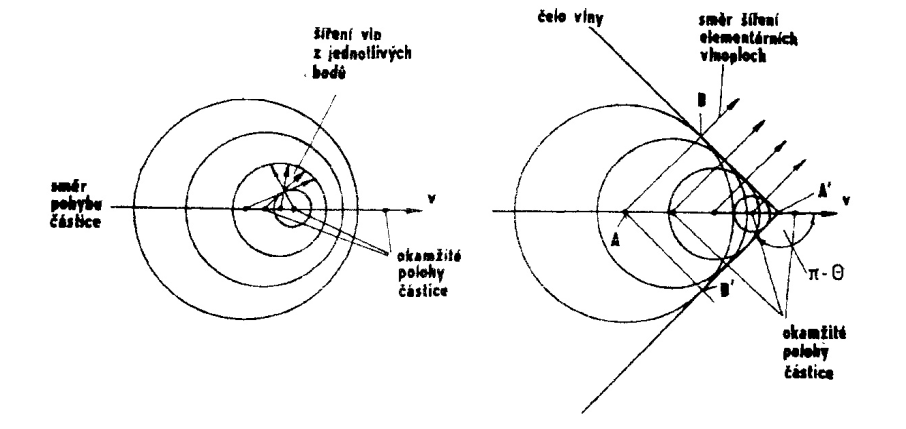
\includegraphics[width=0.8\textwidth]{em4-cerenk1.png}
\caption{Huygensova konštrukcia čela vlny Čerenkovovho žiarenia.}
\label{em4:img:cerenk1}
\end{figure}

Čelo vlny Čerenkovovho žiarenia má tvar plášťa kužeľa s vrcholovým uhlom $2\theta$, pričom pre $\theta$ platí
\begin{equation}
\cos \theta=\dfrac{1}{\beta n}
\end{equation}
Meraním uhlu $\theta$ je možné stanoviť rýchlosť a teda aj energiu častice. Presnosť merania tohto uhlu je teda zviazaná s energetickou rozlišovacou schopnosťou detektoru.

Čerenkovove detektory sú používané hlavne vo fyzike častíc vysokých energií, v oblasti bežných energií sú použiteľné iba na detekciu elektrónov. Ich časová odozva je najrýchlejšia zo všetkých známych typov detektorov, samotná časová konštanta depolarizácie je v ráde pikosekúnd.

Čerenkovove detektory sa rozdeľujú do dvoch kategórií: prvou sú prahové detektory, pretože detekujú iba častice s energiou vyššou ako prahovou. Druhou kategóriou sú diferenciálne detektory, ktoré umožňujú meranie uhlu $\theta$ a určenie rýchlosti častice a teda aj jej energie. Obe varianty sú znázornené na obr. \ref{em4:img:cerenk2}.

\begin{figure}[h]
\centering
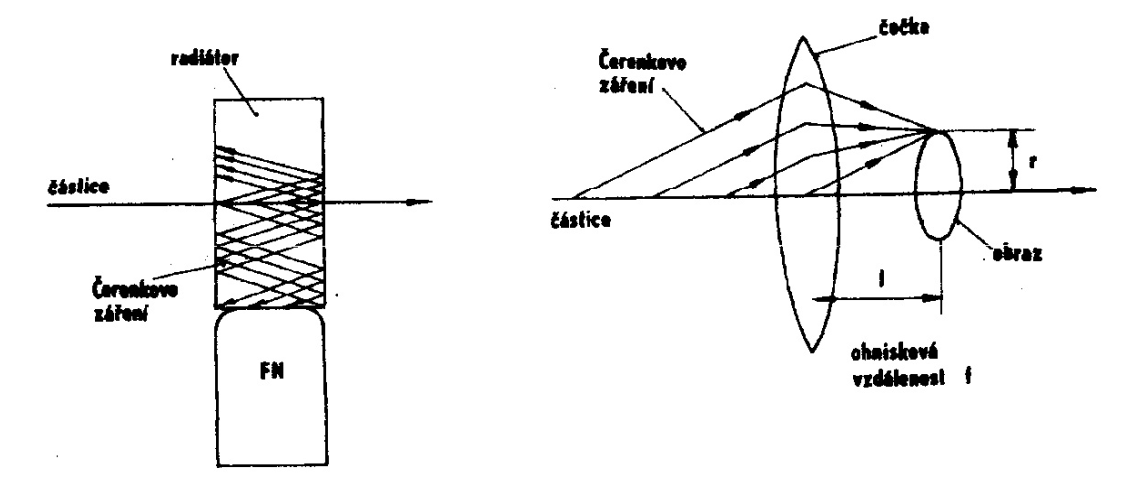
\includegraphics[width=0.8\textwidth]{em4-cerenk2.png}
\caption{Schéma Čerenkovovho prahového (naľavo) a diferenciálneho (napravo) detektoru.}
\label{em4:img:cerenk2}
\end{figure}

Najjednoduchším prahovým detektorom je dielektrikum (radiátor) opticky spojené s fotonásobičom. Akákoľvek nabitá častica s energiou vyššou, než je prahová energia radiátoru, generuje impulzy Čerenkovho žiarenia, ktoré registruje fotonásobič.

Konštrukcia diferenciálneho detektoru na obr. \ref{em4:img:cerenk2} je jednou z mnohých používaných variant tzv. fokusovaného detektoru. Úzky zväzok častíc je orientovaný v smere optickej osi spojky a budí Čerenkovovo žiarenie v plynovom radiátore v priestore pred ňou. Žiarenie je fokusované do krúžku s priemerom $r$, zobrazovaného sa v ohniskovej rovine šošovky. Pre uhol potom platí
\begin{equation}
\theta=\arctan\dfrac{r}{f}
\end{equation}
kde $f$ je ohnisková vzdialenosť šošovky.

Pri detekcii Čerenkovovho žiarenia sa naráža na problém malého počtu vznikajúcich fotónov. Vo vode vzniká cca 200 fotónov na centimeter dráhy ultrarelativistického elektrónu, pri menej optimálnych podmienok je to ešte menej. Sú preto kladené vysoké nároky na vlastnosti fotonásobičov - vysoká kvantová účinnosť fotokatódy pre spektrálnu oblasť Čerenkovovho žiarenia, nízky šum, dobrý optický kontakt fotonásobiča s prostredím či nízka absorpcia žiarenia v prostredí. 

\subsection{Spracovanie signálu}

Prvoradým problémom scintilátorov a detektorov založených na Čerenkovovom žiarení je pokiaľ možno bezstratové zbieranie fotónov, prináležiacich obvykle do blízkej ultrafialovej alebo modrej viditeľnej oblasti svetla, z objemu detektoru a sústrediť ich na vhodný fotosenzitívny prvok, ktorý je v optickom kontakte najčastejšie s jeho podstavou. Pokrytím ostatných stien reflektujúcim materiálom možno po niekoľkonásobných odrazoch dosiahnuť toho, že takmer všetky fotóny emitované v celom objeme detektoru nakoniec vystúpia podstavou.

Označme $n_s$ index lomu scintilátoru a $n_o$ index lomu jej obklopujúceho prostredia. Ak zväzok fotónov dopadá zo scintilátoru na ich rozhranie pod uhlom $\varphi$ (meraný od normály k rozhraniu) väčším než tzv. medzný uhol $\varphi_m=\arcsin \frac{n_o}{n_s}$, dochádza k tzv. totálnemu odrazu. Rozhraním neprejde žiadny fotón do prostredia obklopujúceho scintilátor a plných $100\%$ sa ich odrazí späť do jeho objemu.

V prípade, že je potrebné oddeliť scintilátor od fotonásobiča, používajú sa tzv. svetlovody. Ich funkcia je založená na totálnom odraze od stien. Avšak aj správne navrhnuté svetlovody majú významné straty, v dôsledku ktorých dovedú na katódu iba asi $30$ až $70\%$ vstupujúcich fotónov.

Na optických rozhraniach scintilátor - výstupné okienko - svetlovod - vstupné čelo fotonásobiča nesmie dôjsť k reflexii, ktorá by zmenšila počet fotónov dopadajúcich na fotokatódu. Vzhľadom k tomu, ťe materiály tvoriace rozhranie majú blízke indexy lomu, nemalo by k odrazom dochádzať. Aby sa predišlo aj odrazom spôsobeným nerovnosťou dotykových plôch, vkladá sa medzi detektor a čelo fotonásobiča vrstvička materiálu s blízkym indexom lomu, ktorá medzery zaplní.

\subsection{Fotonásobiče}

Fotonásobiče sú stále najčastejšie používanými fotosenzitívnymi prvkami prevádzajúcimi scintilačné fotóny na impulzný elektrický signál. Fotonásobiče sa skladajú z dvoch hlavných častí: fotokatódy, konvertujúcej fotóny na fotoelektróny, a dynódového násobiaceho systému (viď \ref{em4:img:fotonasobic}).

\begin{figure}[h]
\centering
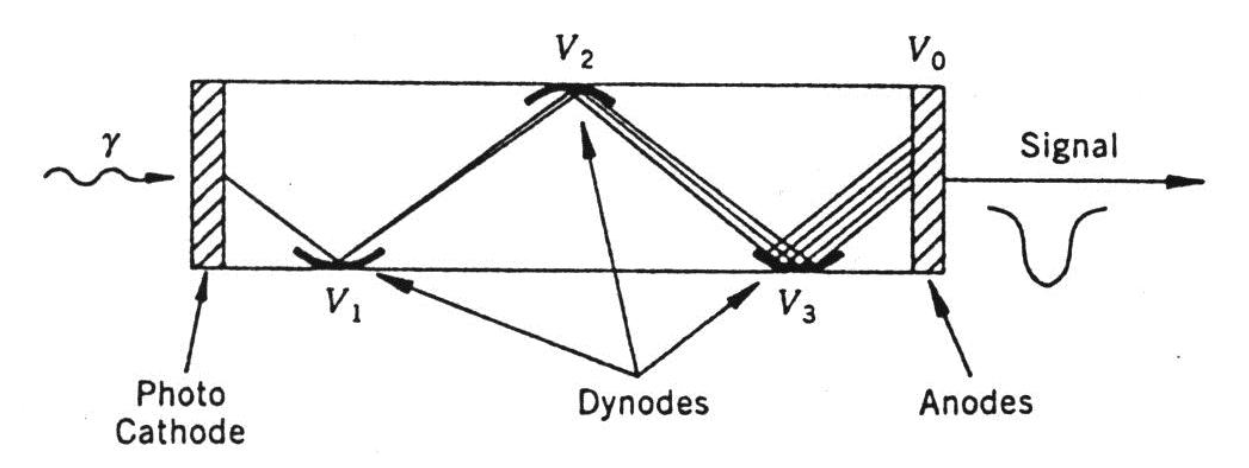
\includegraphics[width=0.8\textwidth]{em4-fotonasobic.png}
\caption{Schéma fotonásobiča. V ľavej časti je znázornená fotokatóda, ktorá konvertuje prichádzajúce gama kvantum na elektrón. Vnútri fotonásobiča sa následne tento elektrón násobí v systéme dynód, pokiaľ nie je dovedený k anóde.}
\label{em4:img:fotonasobic}
\end{figure}

Činnosť fotokatód je založená na vonkajšom fotoelektrickom jave, pri ktorom je uvoľnený elektrón emitovaný do vákua. Aby k javu došlo, je treba, aby energia fotónu bola rovnaká alebo vyššia, ako väzbová energia elektrónu materiálu fotokatódy. Veľkosť väzbovej energie teda určuje dlhovlnnú hranicu spektrálnej charakteristiky fotonásobiča. Krátkovlnná medza je určená v podstate spektrálnou priepustnosťou vstupného okienka fotonásobiča.

Ideálna fotokatóda by mala mať v každom mieste rovnakú citlivosť, v skutočnosti tomu tak nie je a najmä na okrajoch fotokatódy je pozorovateľný aj viac než $20\%$-ný pokles citlivosti. Tento nepríjemný fakt však možno obísť použitím fotonásobiča s priemerom fotokatódy väčším, než je priemer scintilátoru. Podobne, ako nehomogenita fotokatódy, sa prejavuje rôzna účinnosť zberu fotoelektrónov z rôznych miest plochy fotokatódy na prvú dynódu elektrónového násobiaceho systému. K zosilneniu prúdu fotokatódy sa využíva javu sekundárnej emisie. Pri ňom primárny fotón s istou nadprahovou kinetickou energiou pri svojom dopade na povrch kovu s nízkou výstupnou prácou z neho do vákua vyžiari viac, než jeden sekundárny elektrón. Stredný počet vyrazených sekundárnych elektrónov je úmerný energii dopadajúceho elektrónu. Násobiaci systém sa skladá obvykle z 10 až 14 dynód opatrených povlakom z materiálu s veľkým súčiniteľom sekundárnej emisie, zakončený je zbernou elektródou - anódou s najvyšším kladným potenciálom. Dynódy sú tvarom aj vzájomnou geometriou usporiadané tak, aby nedochádzalo k únikom elektrónov zo systému.


\section{Dráhové komory}

Na rozdiel od doteraz preberaných detektorov, ktoré sú schopné registrovať existenciu častíc, rozlíšiť ich od seba, merať tok častíc alebo ich energiu a merať súradnice miesta, ktorým častica prešla, poskytujú dráhové komory viac možností. V týchto detektoroch nabitá častica svojimi ionizačnými účinkami zmení stav náplne komory tak, že sa vytvoria viditeľné stopy dráh nabitých častíc. V subatómovej fyzike sa pracoval a aj pracuje s mnohými typmi dráhových komôr.

\subsection{Jadrové fotoemulzie}

Sú to fotografické emulzie s relatívne veľkou koncentráciou bromidu strieborného (AgBr). Vyrábajú sa vo vrstve silnej až 1 mm a sú pomerne citlivé, takže k vytvoreniu latentného obrazu stačí malá energia. Ak vnikne do tejto emulzie rýchla nabitá častica, zanecháva pozdĺž dráhy svojho pohybu ionizačnú stopu, v ktorej fotochemickou reakciou dochádza k uvoľňovaniu striebra v zrniečkach halogénov striebra rozptýlených v želatíne emulzie.

Jadrové emulzie tvoria v niektorých experimentoch súčasne terčík aj detektor. Zostavujú sa z nich bloky s objemom rádovo litrov až desiatok litrov, ktoré sa ožiarujú časticami. Po vyvolaní sa prezerajú mikroskopom. Na zaregistrovaných stopách možno merať dolet, hustotu ionizácie úmernú počtu vyvolaných zŕn na jednotke dĺžky dráhy a mnohonásobný rozptyl. Z posledného merania možno určiť hybnosť častice.

Dráha nabitej častice s energiou v oblasti minima ionizácie sa javí ako zhluk zrniečok s hustotou asi 300 zrniečok na 1 mm dráhy. Emulzie sa tiež rozmiestňujú vo vhodnom geometrickom usporiadaní okolo terčíku. Z počtu a dĺžky stôp v jednotlivých doskách potom možno stanoviť uhlové a energetické rozdelenie produktov reakcie.

Jadrové emulzie zohrali dôležitú úlohu pri štúdiu jadrových procesov elementárnych častíc na prvých generáciach urýchľovačov a v kozmickom žiarení. Nevýhodou jadrových emulzií sú ich malé rozmery a malá operatívnosť použitia - dráhy častíc sa zviditeľňujú až dodatočne, po vyvolaní, ich vyhodnocovanie je pomalé a pracné. Preto boli postupne vytlačené, predovšetkým bublinkovými komorami, ktoré poskytujú podstatne rýchlejšie a úplnejšie informácie o pohybe a interakciách elementárnych častíc. A teraz sú aj bublinkové komory vytláčané elektronickými detekčnými systémami.

Jadrové emulzie sa však dodnes používajú v niektorých časticových experimentoch, kde je treba veľmi vysoké priestorové rozlíšenie registrovaných dráh častíc, rádovo mikrometre. Často sa používa \quotedblbase sendvičové\textquotedblright ~usporiadanie fotoemulzií v rade vrstiev filmov priložených tesne k sebe, s príp. preložením vrstvami terčíkového materiálu (napr. olova). Toto usporiadanie sa označuje ako ECC (\textit{Emulsion Cloud Chamber}). Vyhodnocovanie fotoemulzií je v moderných detekčných systémoch plne automatizované, prevádza sa mikroskopickým skenovaním, elektronickou digitalizáciou a počítačovým vyhodnotením. 




\subsection{Hmlové komory}

Prvým druhom detektoru, umožňujúcim priebežne zviditeľniť stopy preletu nabitých častíc, bola hmlová komora. Jej hlavnou časťou je uzatvorená komora naplnená plynom s prímesou nasýtených pár. Ak zmeníme podmienky tak, aby sa z nasýtených pár stali pary presýtení, dôjde ku kondenzácii na zrniečkach prachu a tiež na iónoch vytvorených nabitou časticou, ktorá prešla komorou. Pri vhodnom osvetlení možno kvapôčky znázorňujúce stopu častice pozorovať alebo dokonca fotografovať. Hmlové komory delíme na expanzné (Wilsonove) a difúzne.

Vo Wilsonovej komore je presýtenie pár dosiahnuté adiabatickou expanziou. Ak spravíme rýchlu expanziu pracovného priestoru komory, dôjde vplyvom adiabatického rozpínania plynu vo valci k poklesu teploty a prítomné nasýtené pary sa stanú parami presýtenými. Hmlová komora ostáva v presýtenom stave citlivá na registráciu dráh častíc iba po dobu desatín sekundy. Po fotografickom zachytení stôp častíc je treba uviesť komoru do východzieho stavu: prevedie sa spätná kompresia plynu v pracovnom valci, kvapôčky sa vyparia alebo stečú po stenách valca, para sa stane opäť nenasýtenou. Môže potom nastať nový pracovný cyklus expanzia - expozícia - kompresia.

Nevýhodou klasickej Wilsonovej hmlovej komory je krátka citlivá doba registrácie behom pracovného cyklu. Preto bol vyvinutý typ hmlových komôr pracujúcich kontinuálne - difúzne hmlové komory. V difúznej komore sa využíva difúzia pár v plyne s veľkým teplotným gradientom. Ten sa dosiahne zahrievaním jednej dosky, a chladením druhej. Pary alkoholu, vznikajúce v jednej časti komory, difundujú do studenej časti komory. V určitej časti priestoru komory vznikne pásmo, v ktorom nastáva stav presýtených pár. Pary sú neustále dopĺňané kvapkami privádzaného alkoholu, takže difúzna hmlová komora môže v ustálenom stave fungovať nepretržite.



Hmlové komory sa väčšinou umiestňujú do magnetického poľa, ktorého vektor indukcie je kolmý na rovinu, v ktorej pozorujeme, alebo fotografujeme stopy častíc. Dráhy častíc sú potom zakrivené a meraním polomeru krivosti možno určiť náboj a hybnosť častice.

V súčasných experimentoch sa už hmlové komory nevyužívajú.


\subsection{Bublinkové komory}

Bublinková komora je tvorená uzavretou nádobou, ktorá je naplnená kvapalinou zahriatou tesne pod bod varu. Pri expanzii kvapaliny môže vzniknúť nestabilná, prehriata kvapalina s teplotou nad bodom varu. V tomto stave vytvárajú nečistoty alebo ióny vzniklé pri prechode nabitej častice centrá, v ktorých okolí začne kvapalina vrieť, t.j. objavia sa bublinky. Tie možno osvetliť, vyfotografovať, a tým zachytiť dráhu častice.

Ako náplne sa v bublinkových komorách používajú skvapalnené plyny (napr. vodík, deutérium, propán, xenón a freón), podľa povahy experimentu, na ktorý je komora určená.

\begin{figure}[h]
\centering
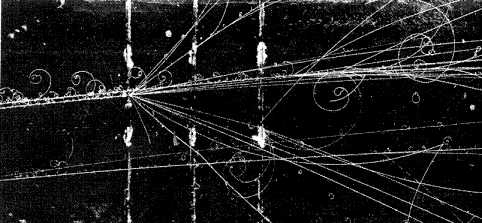
\includegraphics[width=0.7\textwidth]{em4-hmlova.jpg}
\caption{Ukážka fotografickej snímky z bublinkovej komory. Primárna častica (protón) z urýchľovača, prilietava zľava, zanecháva ionizačnú stopu a potom zrážkou produkuje ďalšie častice, z ktorých tie elektricky nabité zanechávajú opäť ionizačné stopy. Komora je vložená do magnetického poľa, takže podľa znamienka náboja sa dráhy častíc zakrivujú vľavo (záporné častice) alebo vpravo (kladné častice).}
\label{em4:img:hmlova}
\end{figure}

 Bublinková komora slúži súčasne ako terčík  aj ako detektor. Objemy týchto komôr môžu dosahovať až $15\:\unit{m^3}$. Veľké komory mávajú guľový tvar, menšie sú natiahnuté s dĺžkou do dvoch metrov. Umiestňujú sa do magnetického poľa a fotografovanie dráh sa prevádza niekoľkými kamerami z rôznych smerov, aby bolo možné stopu priestorovo zrekonštruovať. Na snímkoch je možné merať krivosť dráh, uhly, pod ktorými sú častice z miesta interakcie vysielané, a ionizáciu. Z týchto dát dokážeme stanoviť hybnosť častíc, znamienko náboja a druh častice. Pri dostatočne pomalých časticiach je možné merať aj dolet.
 
 Komory pracujú v zväzkoch častíc získaných z urýchľovačov. V súčasnej dobe sa už menej používajú. Existujú však špeciálne typy komôr malých rozmerov, kde sa dosahuje veľmi dobré priestorové rozlíšenie $\sim 15$ mm.

\subsection{Iskrové komory}

Iskrová komora je jedno z prvých zariadení v časticovej fyzike, ktore slúžilo na detekciu elektricky nabitých častíc. Boli prevažne používané v rokoch 1940 - 1960.

Táto komora pozostáva z kovových dosiek, ktoré sú umiestnené v tlakovo uzavretej komore vyplnenej inertným plynom s vhodnými vlastnosťami (napr: hélium, argón, neón...), viď obr.\ref{em4:img:spark}. Dvojice týchto elektród sú striedavo napojené na vysokom potenciály a uzemnené. Pre vzdialenosť elektród asi 8 mm sa používa napätie asi 10 kV na dobu $0,2\:\unit{\mu s}$. 

Pri prechode nabitej častice cez iskrovú komoru táto častica ionizuje plyn nachádzajúci sa v komore medzi platňami. Za normálnych okolnosti táto ionizácia nie je pozorovateľná. Avšak ak aplikujeme dostatočne veľké napätie medzi susednými platňami predtým ako ionizácia vymizne, tak môžme pozorovať iskry, ktoré sa tvoria pozdĺž trajektórie častice. Týmto spôsobom je v našich silách pozorovať danú trajektóriu príslušnej nabitej častice. Toto vysoké napätie však nemôže byť udržiavané permanentne medzi platňami pretože by to mohlo viesť k formovaniu elektrických oblúkov a priebežnému vybíjaniu zdroja.

\begin{figure}[h]
\centering
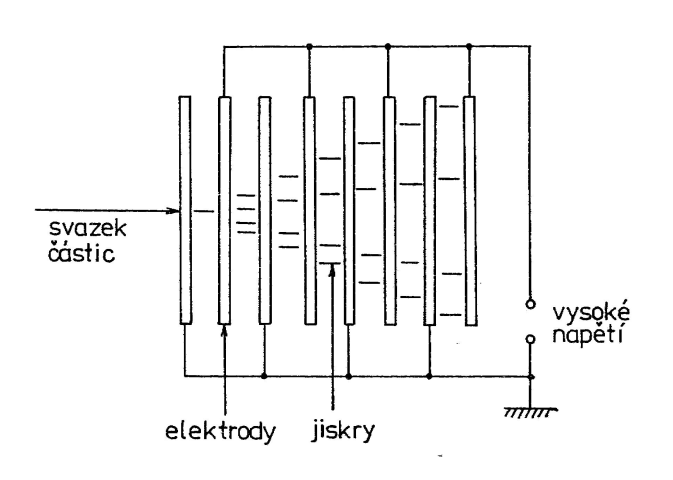
\includegraphics[width=0.6\textwidth]{em4-spark.png}
\caption{Schéma iskrovej komory.}
\label{em4:img:spark}
\end{figure}

Na kontrolu toho, kedy bude dané napätie aplikované, je potrebný ďalší detektor, ktorý bude rozhodovať o tom, kedy zapnúť dané napätie medzi platňami. Tento detektor často obsahuje scintilátory, ktoré sú umiestnené na vrchnej a spodnej strane komory. 
Keď trigrový systém detektora pocíti, že daným detektorom prešla nabitá častica, spustí sa spínač, ktorý privedie na platne vysoké napätie.

Hlavné medzníky v živote iskrovej komory:
\begin{itemize}
 \item  \textbf{1949}: Keuffel prvýkrát pozoruje elektrický výboj medzi paralelnými platňami vznikajúci pozdĺž trajektórie kozmického žiarenia.
 \item  \textbf{1955}: Hennings and Bagge spravili pár vylepšení. Použili viacej paralelných dosiek, vylepšili iskru použitím argónu alebo alkoholu a odfotili stereo fotografiu.
 \item  \textbf{1957}: Harwell, Cranshaw a de Beer vyvinuli trigger systém.
 \item  \textbf{1959}: Fukui a Migamoto predstavujú možnosť pozorovania viacej ako len jednej častice naraz, použitie vzázneho plynu a aplikovanie vysokého napätia ešte rýchlejšie.
 \item  \textbf{1963}: Alikhanian prišiel z myšlienkou vytvorenia komory, kde medzery medzi platňami budú také široké, že bude možné pozorovať trajektóriu častice, ktorá bude dlhá až 20 cm.
\end{itemize}

Používanie dráhových komôr sa postupne obmedzuje vzhľadom k relatívne veľmi náročnému spracovaniu dát o dráhach častíc. Pre daný experiment je totiž nutné vyvolať rádovo $10^6$ fotografických snímkov, každý z nich prezrieť a vybrať tie, ktoré zachytávajú skúmaný proces. Keďže táto činnosť vyžaduje veľký počet pracovných síl, stavajú sa miesto dráhových komôr veľké a zložité systémy detektorov dovoľujúce jednoduchšiu analýzu experimentu.


\subsection{Detektor prechodového žiarenia}

Detektor prechodového žiarenia (TRT - Transition radiation detector) je dráhový detektor využívajúci prechodové žiarenie. Obsahuje stovky tisíc plynom naplnených tenkých slamiek\footnote{česky brčka} s priemerom 4 mm. Vnútri každej slamky je veľmi presne vycentrovaný pozlátený wolfrámový drôtik s priemerom 0,03 mm.

Slamky sú obklopené polypropylénovou penou, ktorá plní funkciu radiátoru prechodového žiarenia. Prechodové žiarenie je veľmi slabé žiarenie emitované rýchlymi časticami pri prechode rozhraním dvoch prostredí s rôznymi indexmi lomu. Pravdepodobnosť emisie prechodového žiarenia je daná hmotnosťou častice, ktorá emisiu spôsobuje, v závislosti na veľkosti rýchlosti\footnote{napr. pión, ktorý má veľkosť rýchlosti rovnakú ako elektrón, bude menej emitovať žiarenie.}.

\begin{figure}[h]
\centering
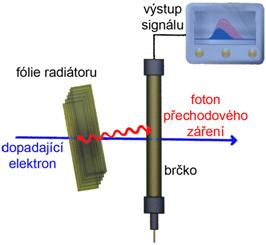
\includegraphics[width=0.4\textwidth]{em4-prechod.jpg}
\caption{Schéma princípu detektoru prechodového žiarenia.}
\label{em4:img:prechod}
\end{figure}

Častica prechádzajúca slamkou ionizuje plyn, čo sa prejaví vznikom elektrických pulzov na elektródach. Medzi slamku a centrálny drôtik je totiž pripojené vysoké napätie. Elektróny vzniknuté ionizáciou vytvoria elektrónovú lavínu, ktorá sa prejaví vznikom elektrického prúdu na výstupných elektródach detektoru. Časový okamžik, v ktorom bol pulz zaregistrovaný systémom, poskytuje určenie polohy týchto častíc s presnosťou 0,15 mm. Slamky teda fungujú ako plynové detektory.

TRT umožňuje odlíšiť elektróny od ťažkých častíc (napr. piónov). Elektróny totiž s ďaleko väčšou pravdepodobnosťou emitujú fotóny prechodového žiarenia než ťažké častice. K tejto emisii dochádza pri prechode elektrónov vrstvami radiátoru. Odlíšenie elektrónov od ťažkých častíc sa využíva v detektore ATLAS v CERNe.

Na meranie hybnosti je TRT kombinovaný s polovodičovými detektormi: TRT dokončuje identifikáciu elektrónov. TRT tiež umožňuje samostatné meranie hybnosti, ale s menšou presnosťou. Detektor TRT je zostavený z troch častí - z dvoch koncových častí s radiálnymi slamkami (v každej koncovej časti je ich 200 000) a jednej centrálnej valcovej časti so slamkami orientovanými v smere osi (tu je asi 100 000 slamiek). 


\end{document}